\chapter{Montaje y Ensamblado}
En todo el proceso de montaje, deberemos de ser extremadamente cautelosos, a fin de evitar errores de unión que comprometerán la integridad estructural o la aerodinámica, echando a perder el perfil.

Antes del montaje al que vamos a proceder, todos los elementos han pasado por un proceso de corte y conformado, donde se han empleado herramientas adecuadas, de calidad y con operarios capacitados.

\section{Proceso}

\subsection{Paso Previo: Preparación de las Costillas en Forma de Perfil Aerodinámico}
Dos de las tres costillas (trasera y delantera) contarán con perforaciones para permitir que la estructura sea accesibles. Para esto, realizamos una perforación rectangular (ancho por alto: $50\times180 \, [\text{mm}]$) en dichas costillas.

Por otro lado, la costilla intermedia y la delantera cuentan con un orificio circular de radio 80 [mm], para poder introducir por su interior el tubo de soporte, que sostendrá a toda la estructura.

Todas las costillas contarán con bordones, sobre los que se apoyarán los larguerillos delanteros y traseros, colocados dos a dos sobre el intradós y el extradós, separados entre sí 260 [mm], y con longitud y profundidad de 40 [mm] y 14 [mm], respectivamente.

Por último, también hay bordones de longitud 20 [mm] para el revestimiento.

\subsection{Primer Paso: Tubo de Soporte}
El tubo de soporte facilita la orientación y sustenta la estructura. Para esto, curvaremos una chapa, obteniendo un tubo de 80 [mm].

Posteriormente, trazamos una generatriz sobre el tubo, donde marcaremos la separación de las costillas (400 [mm]), desde el extremo delantero hacia delante.

Ver figura \ref{fig:primer}.

%===============================================================================================================
%                                                   PRIMER PASO
%===============================================================================================================
\begin{figure}[!htb]
\centering
\begin{tikzpicture}[lablum/.style 2 args={label=below:#1 #2,name=img-#1},
marr/.style={line width=1mm,-latex}]
 \matrix[column sep=1cm,row sep=5mm] (mat)
 { \node[lablum={a}{}]{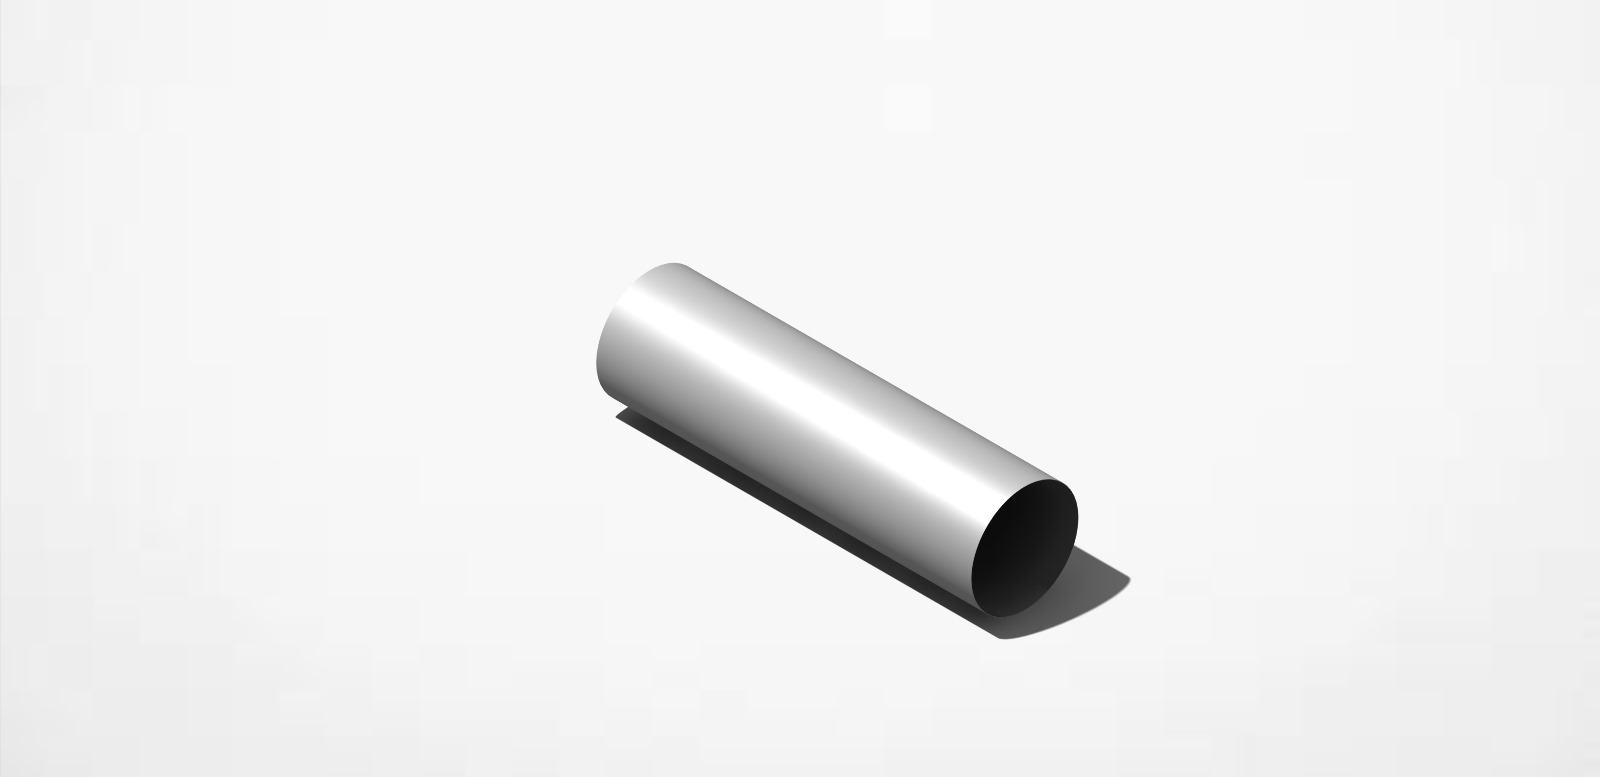
\includegraphics[width=8cm]{Figures/Montaje/1.jpg}};
 & \node[lablum={b}{}]{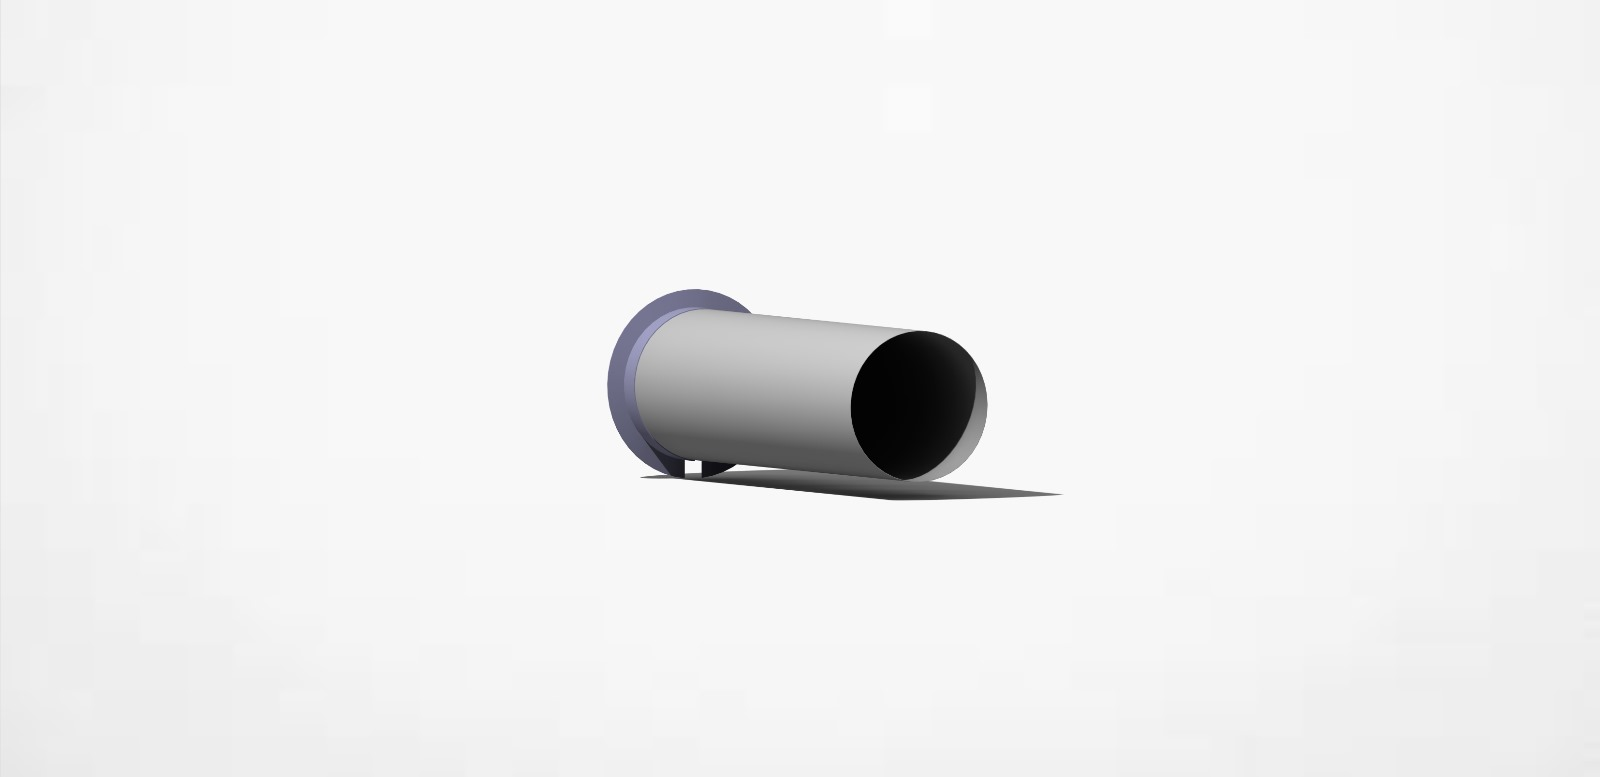
\includegraphics[width=2cm]{Figures/Montaje/2.jpg}};\\
 & \node[lablum=c]{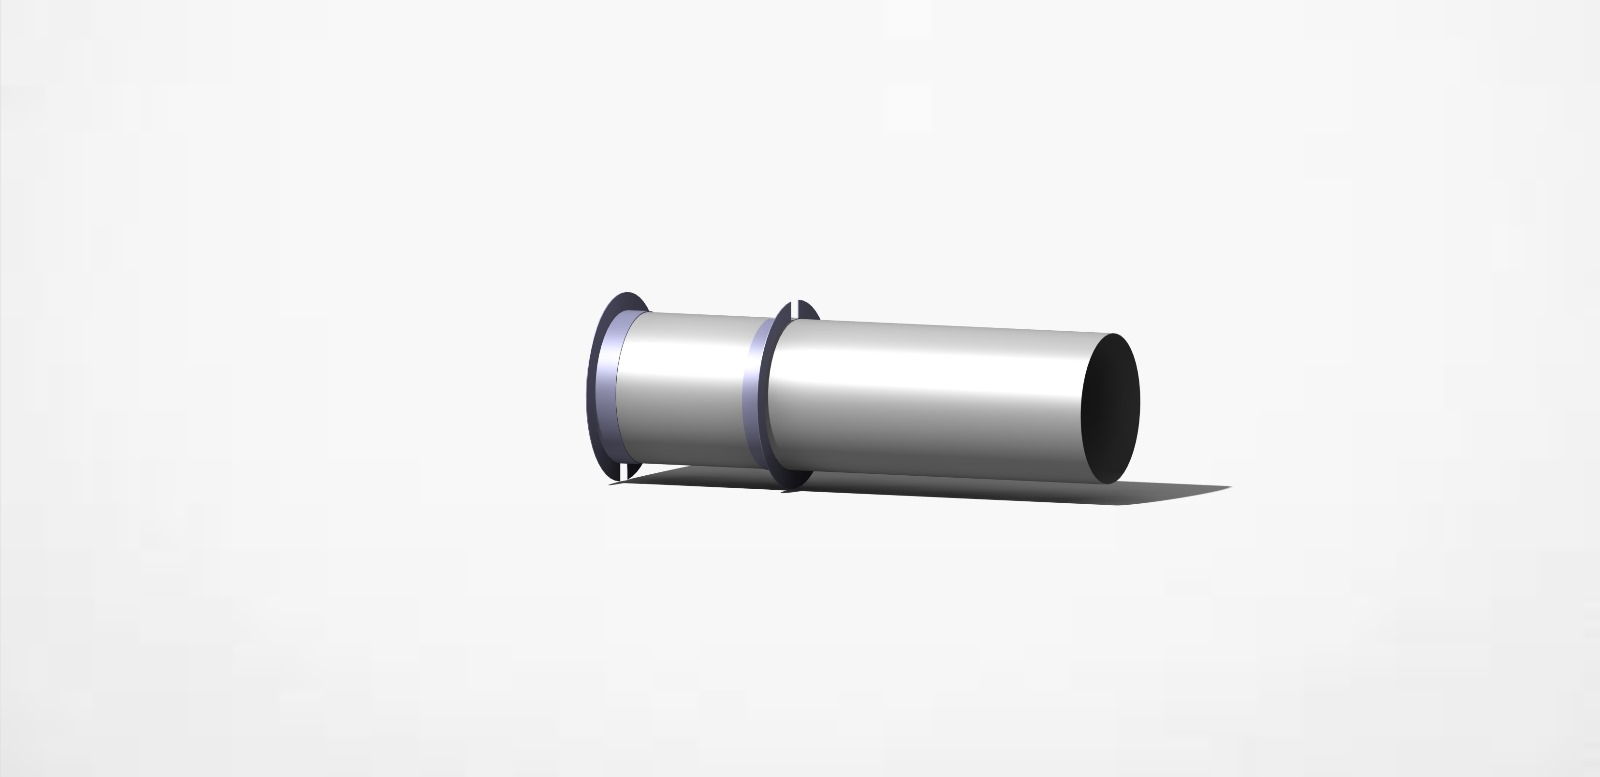
\includegraphics[width=2cm]{Figures/Montaje/3.jpg}};\\
 };
 \draw[marr] (img-a) -- (img-b);
 \draw[marr] ([xshift=1mm]img-b.south east) coordinate (aux) 
 -- (img-c.north-|aux);

\end{tikzpicture}
\caption{Primer Paso. \label{fig:primer}}
\end{figure}
%===============================================================================================================


\subsection{Segundo Paso: Introducción del Sombrerete Trasero}
Colocamos sobre el extremo del tubo de soporte el primer sombrerete, con las solapas hacia el interior del tubo. Se unirá mediante soldadura oxiacetilénica con material de aporte.

Ver figura \ref{fig:seg}.
%===============================================================================================================
%                                                   SEGUNDO PASO
%===============================================================================================================
\begin{figure}[!htb]
\centering
\begin{tikzpicture}[lablum/.style 2 args={label=below:#1 #2,name=img-#1},
marr/.style={line width=1mm,-latex}]
 \matrix[column sep=1cm,row sep=5mm] (mat)
 { \node[lablum={a}{}]{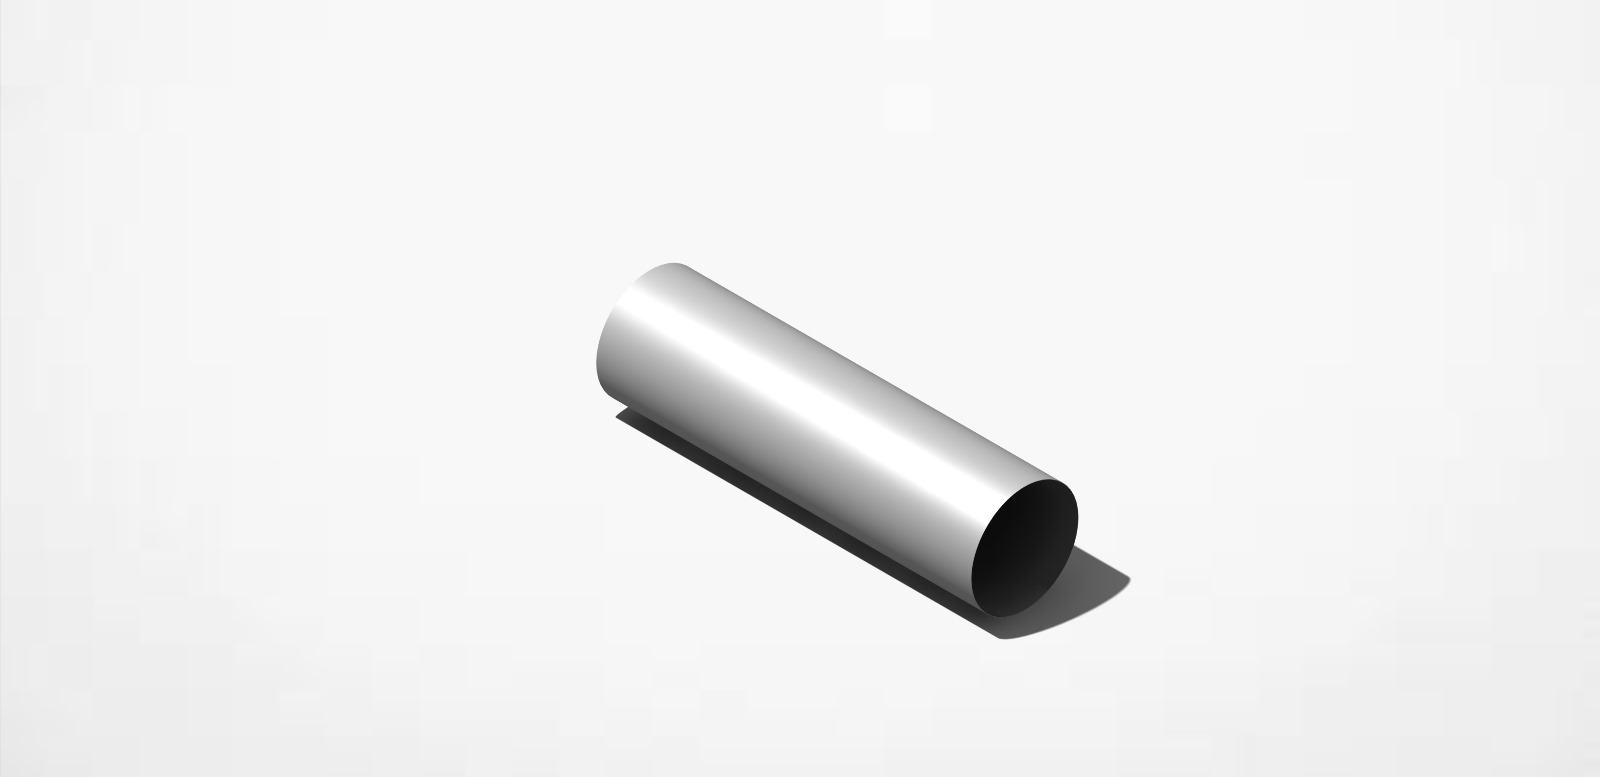
\includegraphics[width=2cm]{Figures/Montaje/1.jpg}};
 & \node[lablum={b}{}]{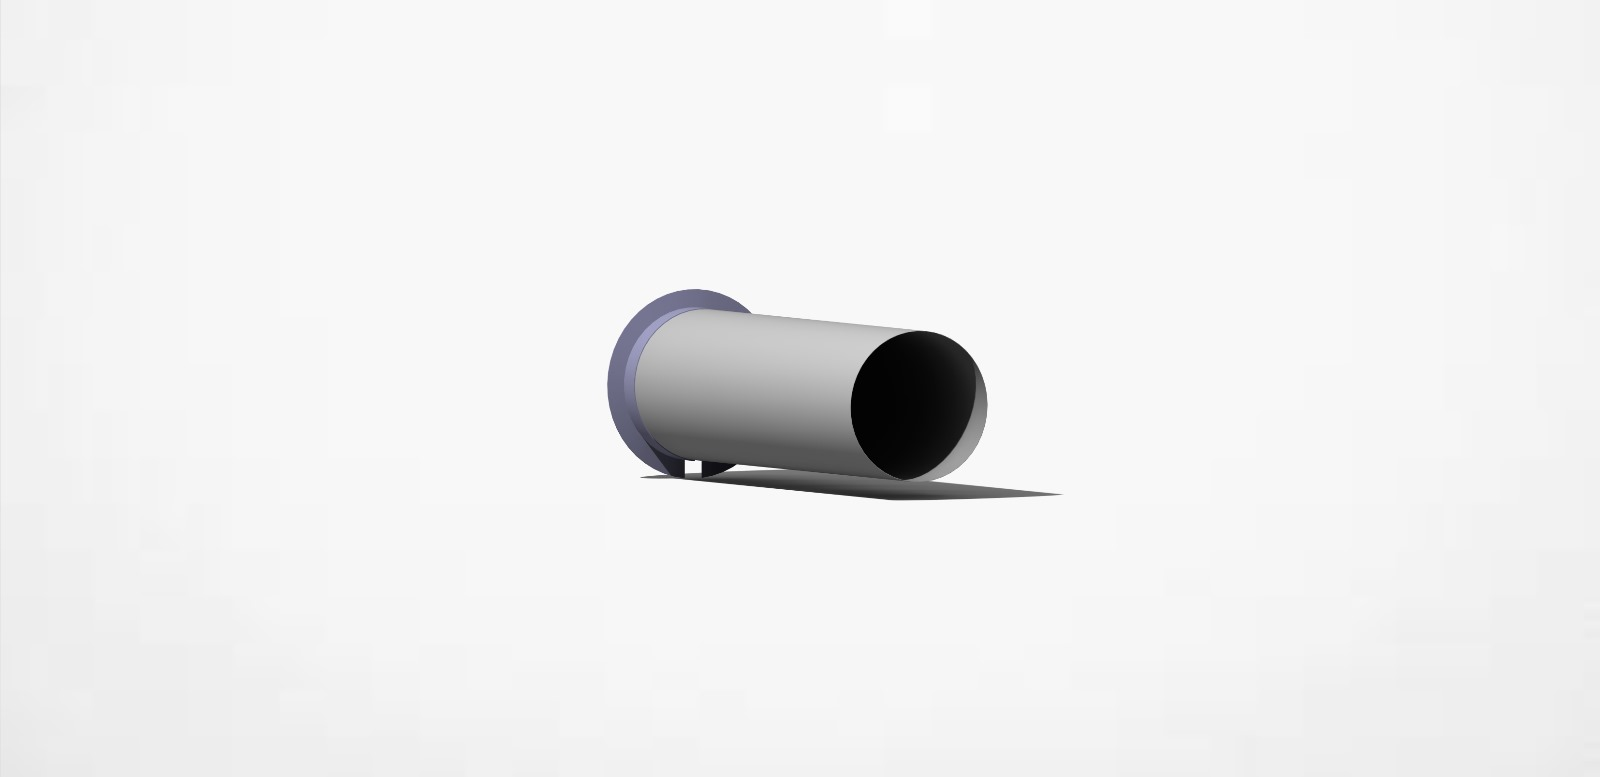
\includegraphics[width=8cm]{Figures/Montaje/2.jpg}};\\
 & \node[lablum=c]{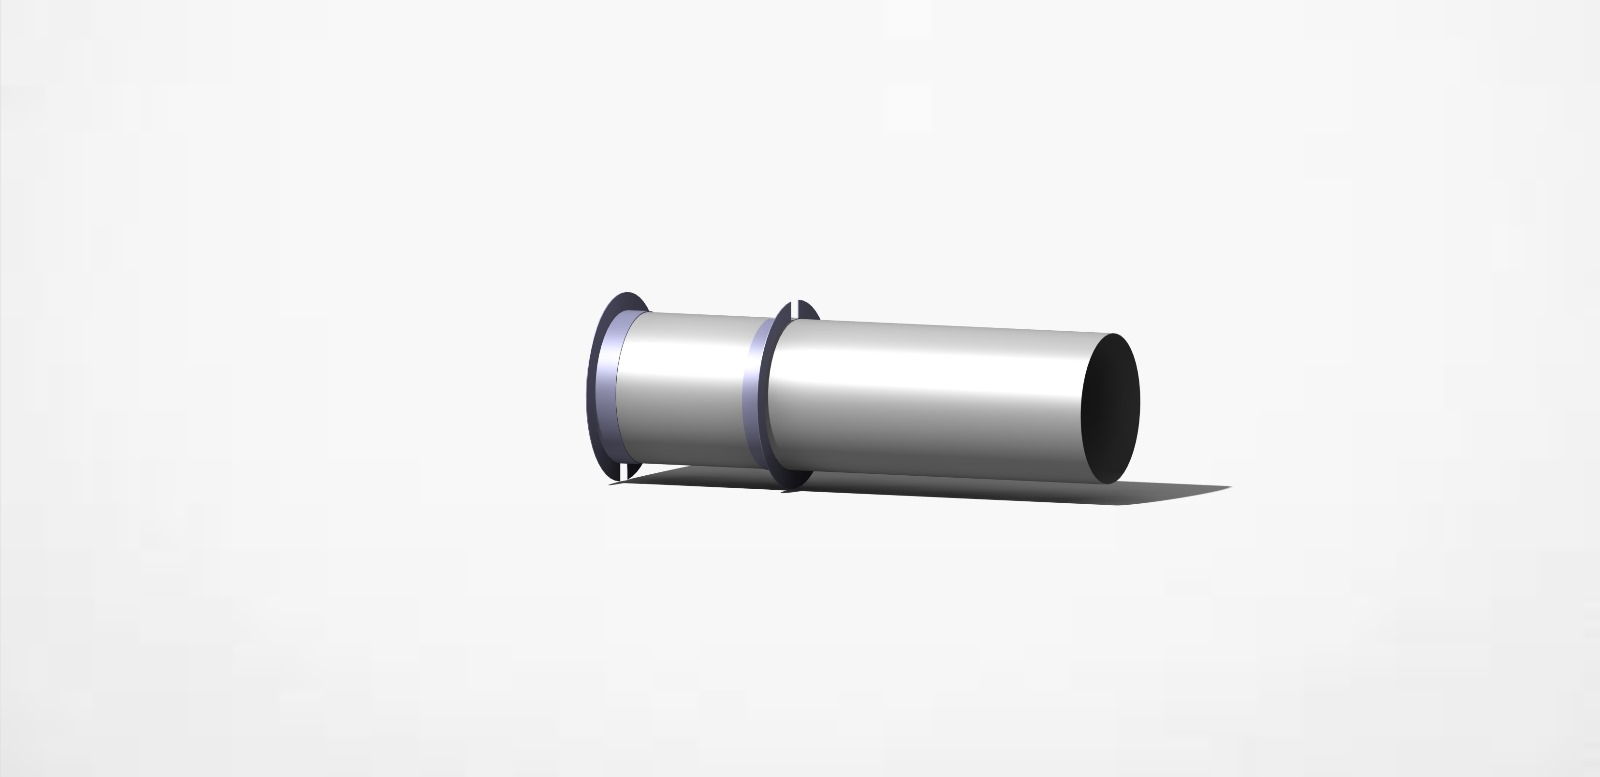
\includegraphics[width=2cm]{Figures/Montaje/3.jpg}};\\ 
 };
 \draw[marr] (img-a) -- (img-b);
 \draw[marr] ([xshift=1mm]img-b.south east) coordinate (aux) 
 -- (img-c.north-|aux);

\end{tikzpicture}
\caption{Segundo Paso. \label{fig:seg}}
\end{figure}
%===============================================================================================================


\subsection{Tercer Paso: Introducción del Sombrerete Intermedio}
Análogo al paso anterior, pero orientando las solapas hacia el primer sombrerete.

Ver figura \ref{fig:ter}

%===============================================================================================================
%                                                   TERCER PASO
%===============================================================================================================
\begin{figure}[!htb]
\centering
\begin{tikzpicture}[lablum/.style 2 args={label=below:#1 #2,name=img-#1},
marr/.style={line width=1mm,-latex}]
 \matrix[column sep=1cm,row sep=5mm] (mat)
 {  & \node[lablum={b}{}]{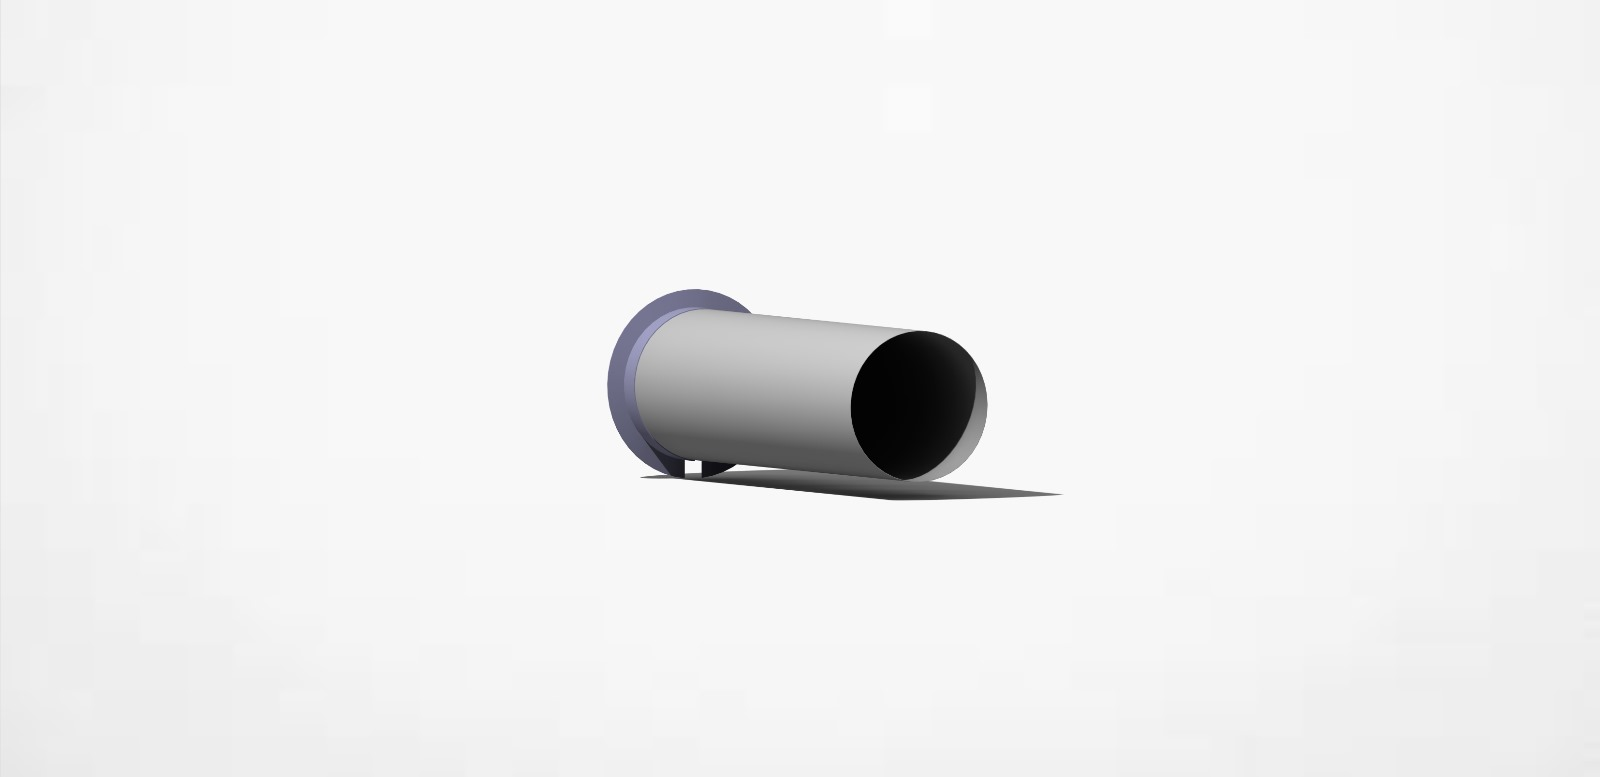
\includegraphics[width=2cm]{Figures/Montaje/2.jpg}};\\
 \node[lablum=d]{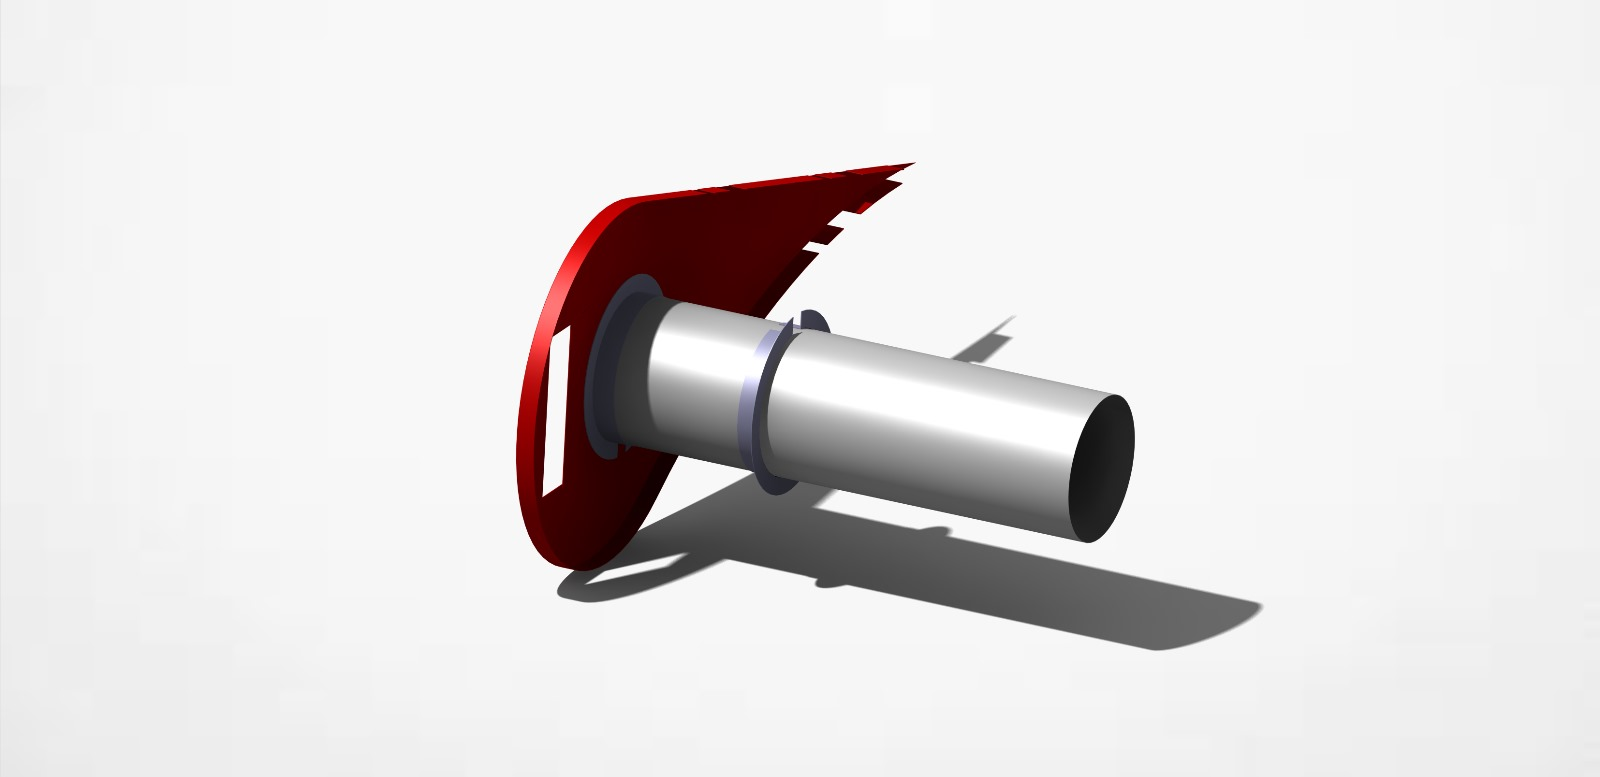
\includegraphics[width=2cm]{Figures/Montaje/4.jpg}};  & \node[lablum=c]{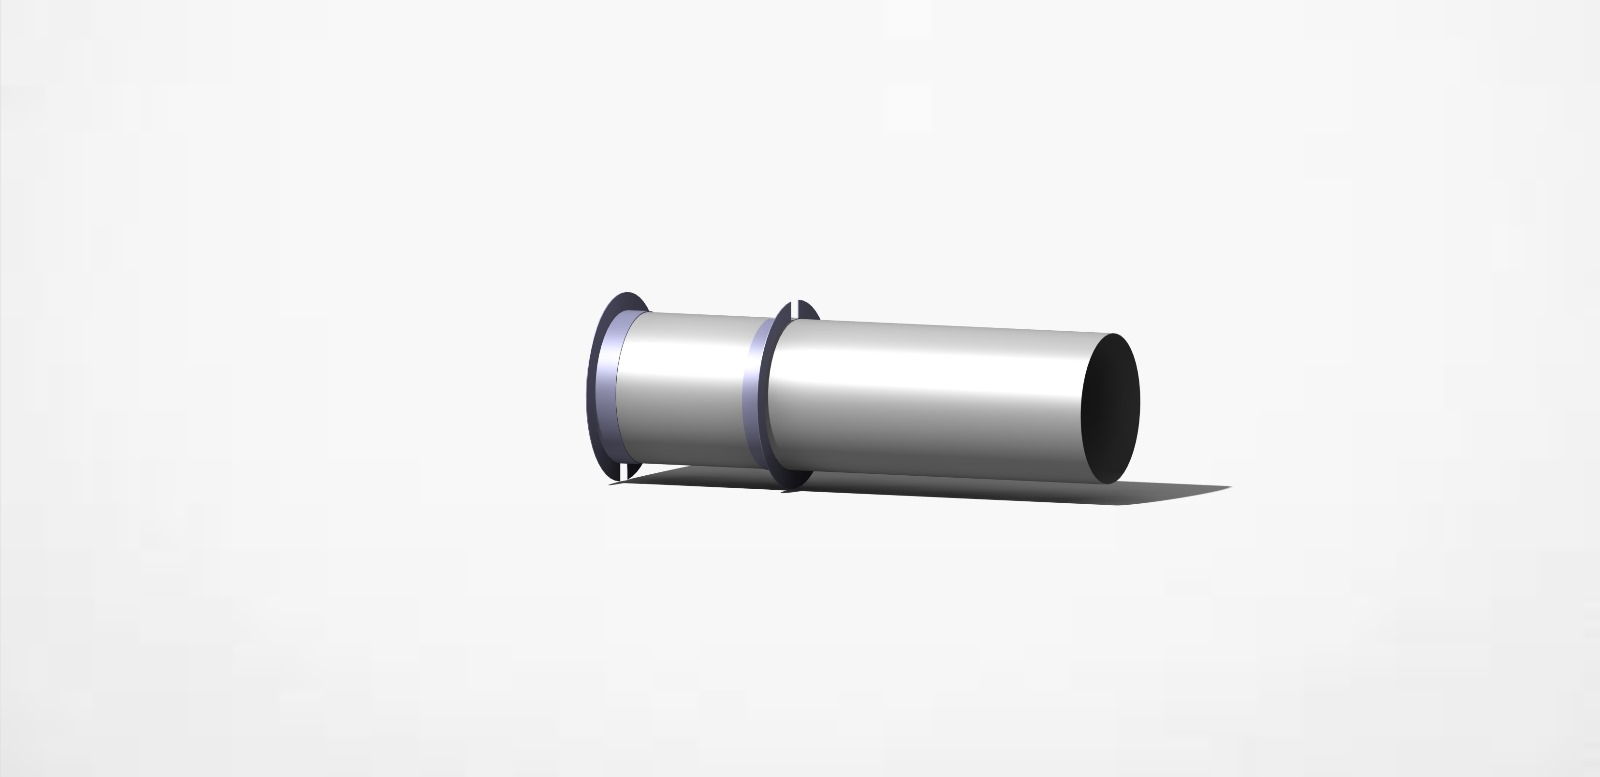
\includegraphics[width=8cm]{Figures/Montaje/3.jpg}};\\
 };
 \draw[marr] ([xshift=1mm]img-b.south east) coordinate (aux) 
 -- (img-c.north-|aux);
 \draw[marr] (img-c) -- (img-d);
\end{tikzpicture}
\caption{Tercer Paso. \label{fig:ter}}
\end{figure}
%===============================================================================================================

\pagebreak
\subsection{Cuarto Paso: Introducción de la Costilla Trasera}
Colocamos la costilla trasera (la única sin perforar) sobre el primer sombrerete (la que está en el extremo del tubo), y trazamos, sobre la parte interior de ella, la posición del sombrerete, para realizar, posteriormente, la unión de sendas piezas mediante un revestimiento con caña maciza y cabeza universal.

La costilla quedará orientada hacia el interior de la estructura, al estar colocada en el exterior del sombrerete.

Ver figura \ref{fig:cua}.

%===============================================================================================================
%                                                   CUARTO PASO
%===============================================================================================================
\begin{figure}[!htb]
\centering
\begin{tikzpicture}[lablum/.style 2 args={label=below:#1 #2,name=img-#1},
marr/.style={line width=1mm,-latex}]
 \matrix[column sep=1cm,row sep=5mm] (mat)
 { \node[lablum=d]{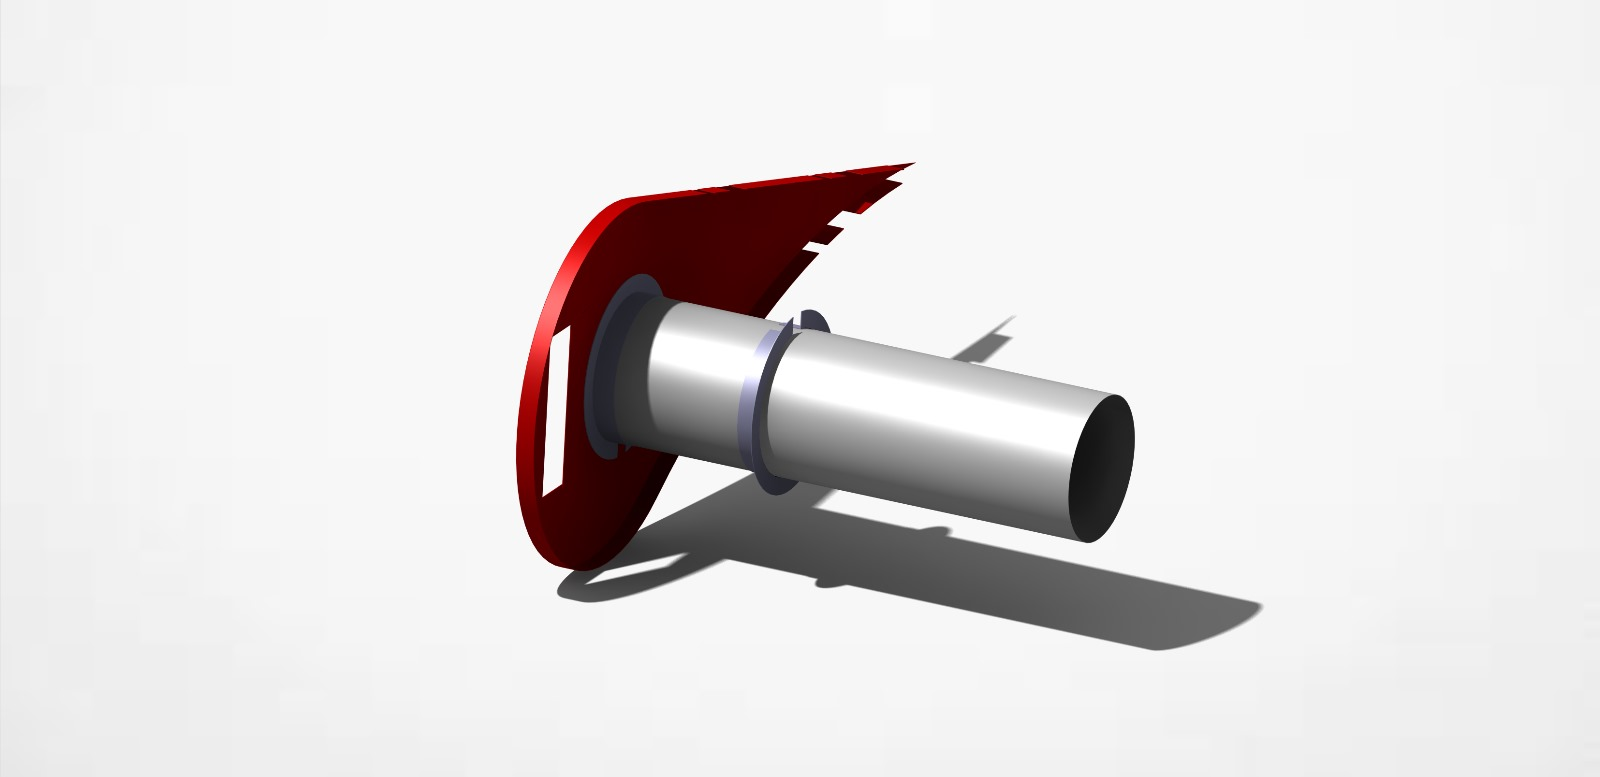
\includegraphics[width=8cm]{Figures/Montaje/4.jpg}};  & \node[lablum=c]{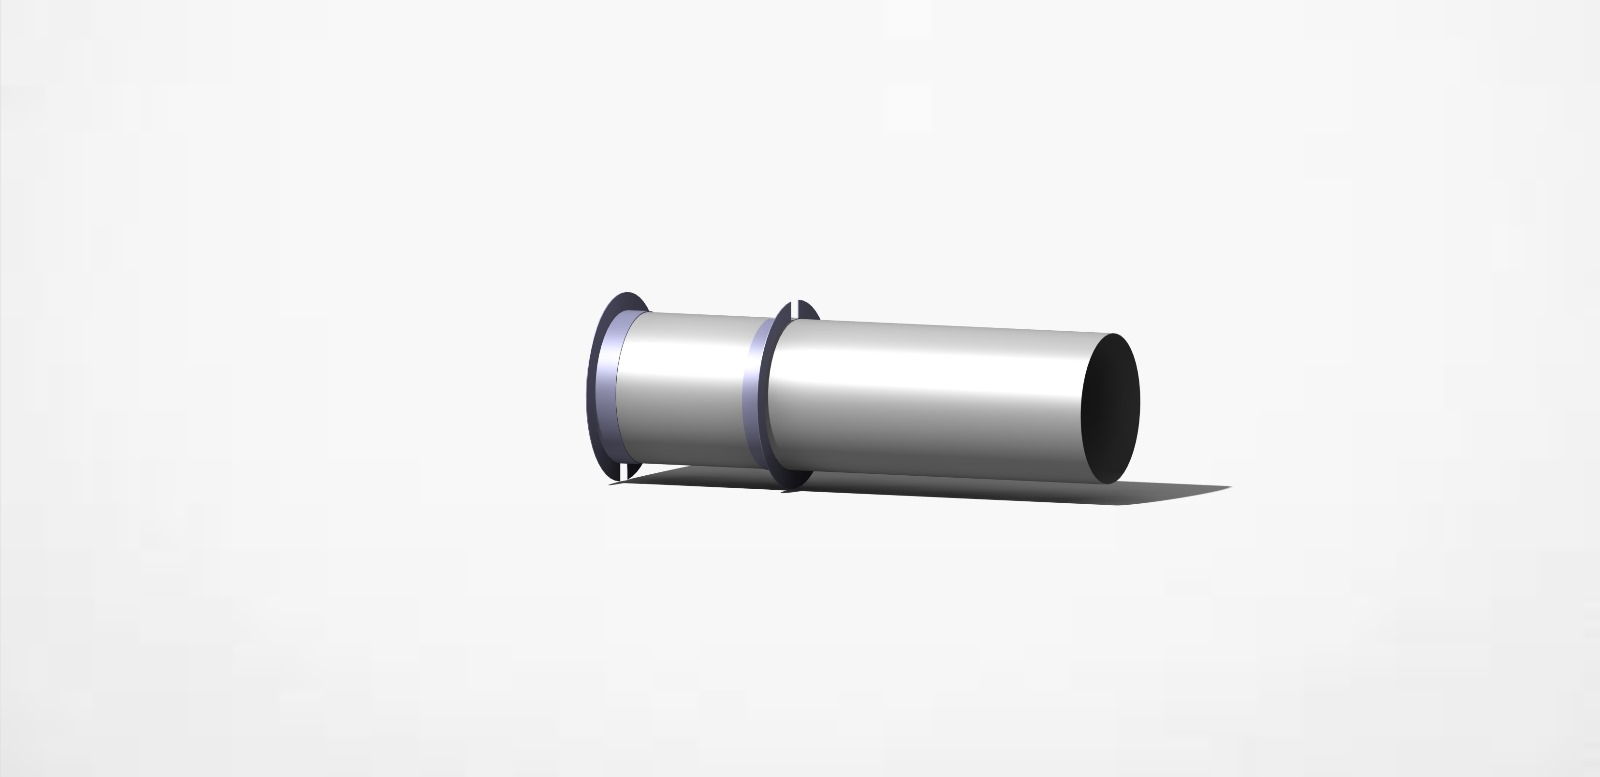
\includegraphics[width=2cm]{Figures/Montaje/3.jpg}};\\
 \node[lablum=e]{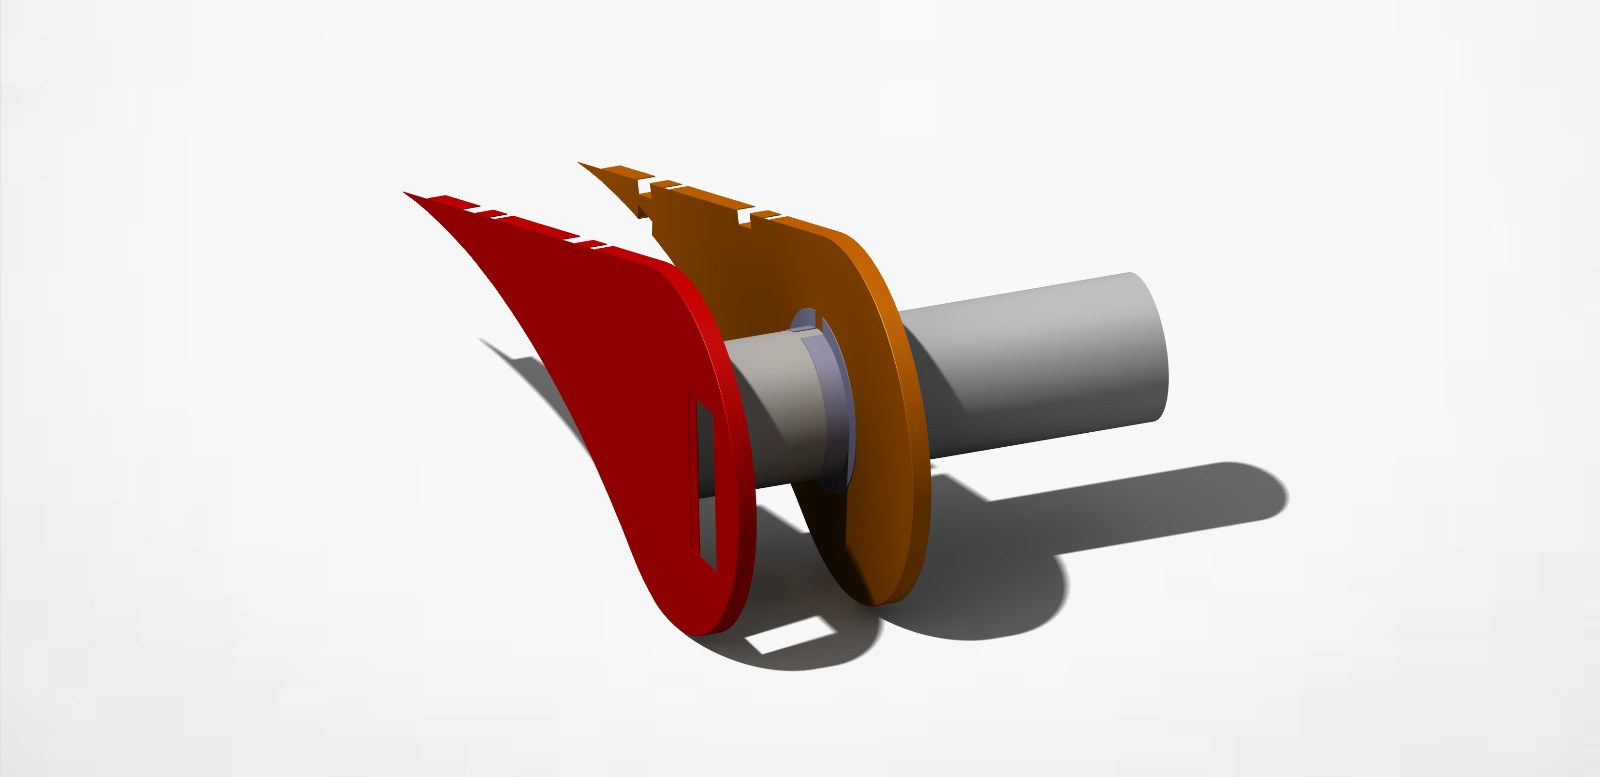
\includegraphics[width=2cm]{Figures/Montaje/5.jpg}};
 & \\
 };
 \draw[marr] (img-c) -- (img-d);
  \draw[marr] ([xshift=-1mm]img-d.south west) coordinate (aux) 
 -- (img-e.north-|aux);
\end{tikzpicture}
\caption{Cuarto Paso. \label{fig:cua}}
\end{figure}

\begin{nota}{Comentario sobre los Próximos Pasos}{}
    Antes de proceder con el Quinto Paso, apoyaremos sobre la mesa de trabajo la parte recta del perfil de trabajo (el correspondiente con el extradós). Haremos esto con el fin de garantizar que todas las costillas queden alineadas correctamente.
\end{nota}
%===============================================================================================================

\pagebreak

\subsection{Quinto Paso: Introducción de la Costilla Intermedia}
Análogo al paso anterior.

Ver figura \ref{fig:qui}.
%===============================================================================================================
%                                                   QUINTO PASO
%===============================================================================================================
\begin{figure}[!htb]
\centering
\begin{tikzpicture}[lablum/.style 2 args={label=below:#1 #2,name=img-#1},
marr/.style={line width=1mm,-latex}]
 \matrix[column sep=1cm,row sep=5mm] (mat)
 { \node[lablum=d]{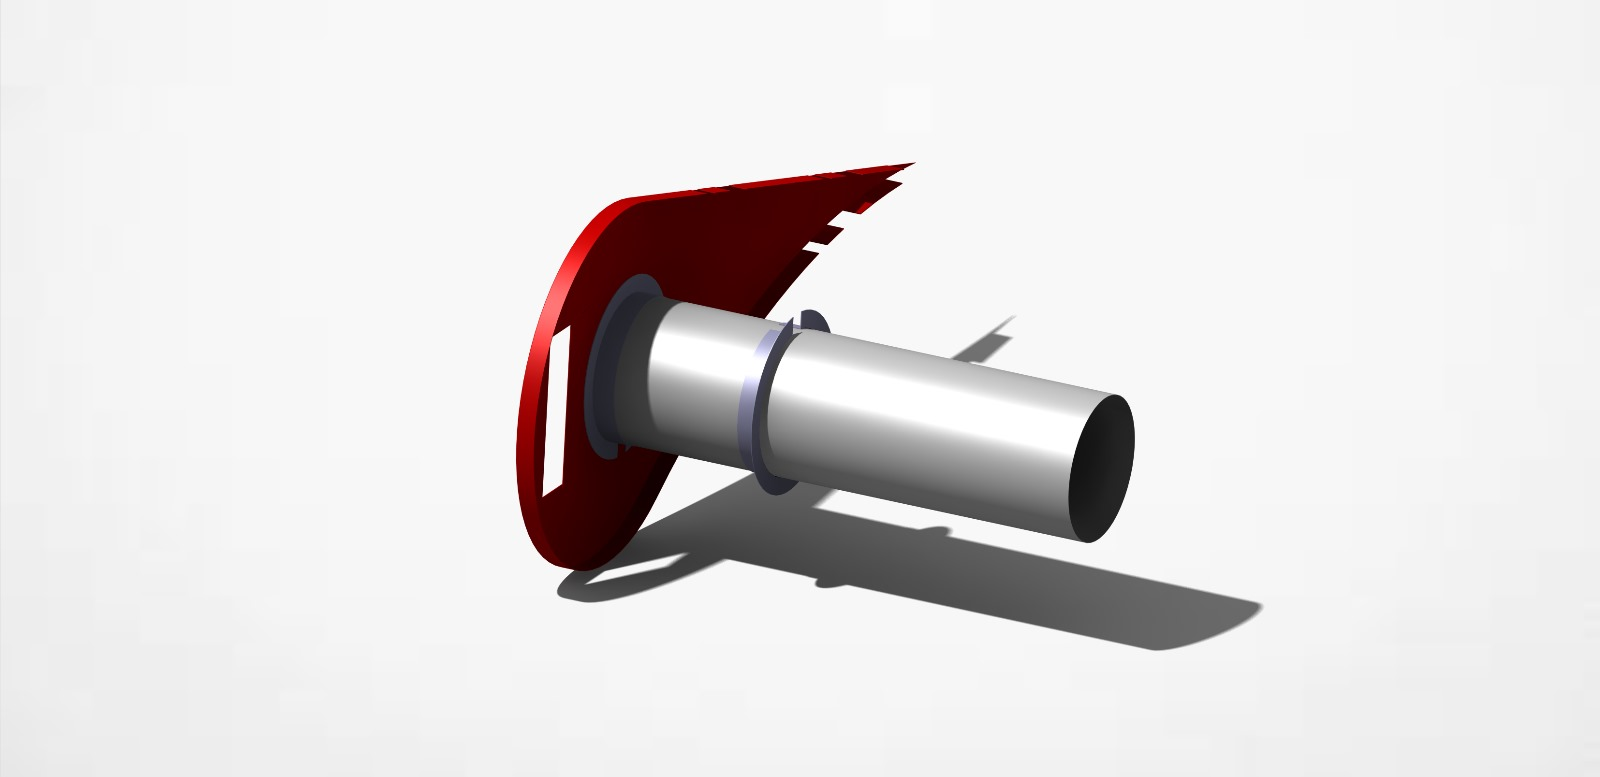
\includegraphics[width=2cm]{Figures/Montaje/4.jpg}}; \\
 \node[lablum=e]{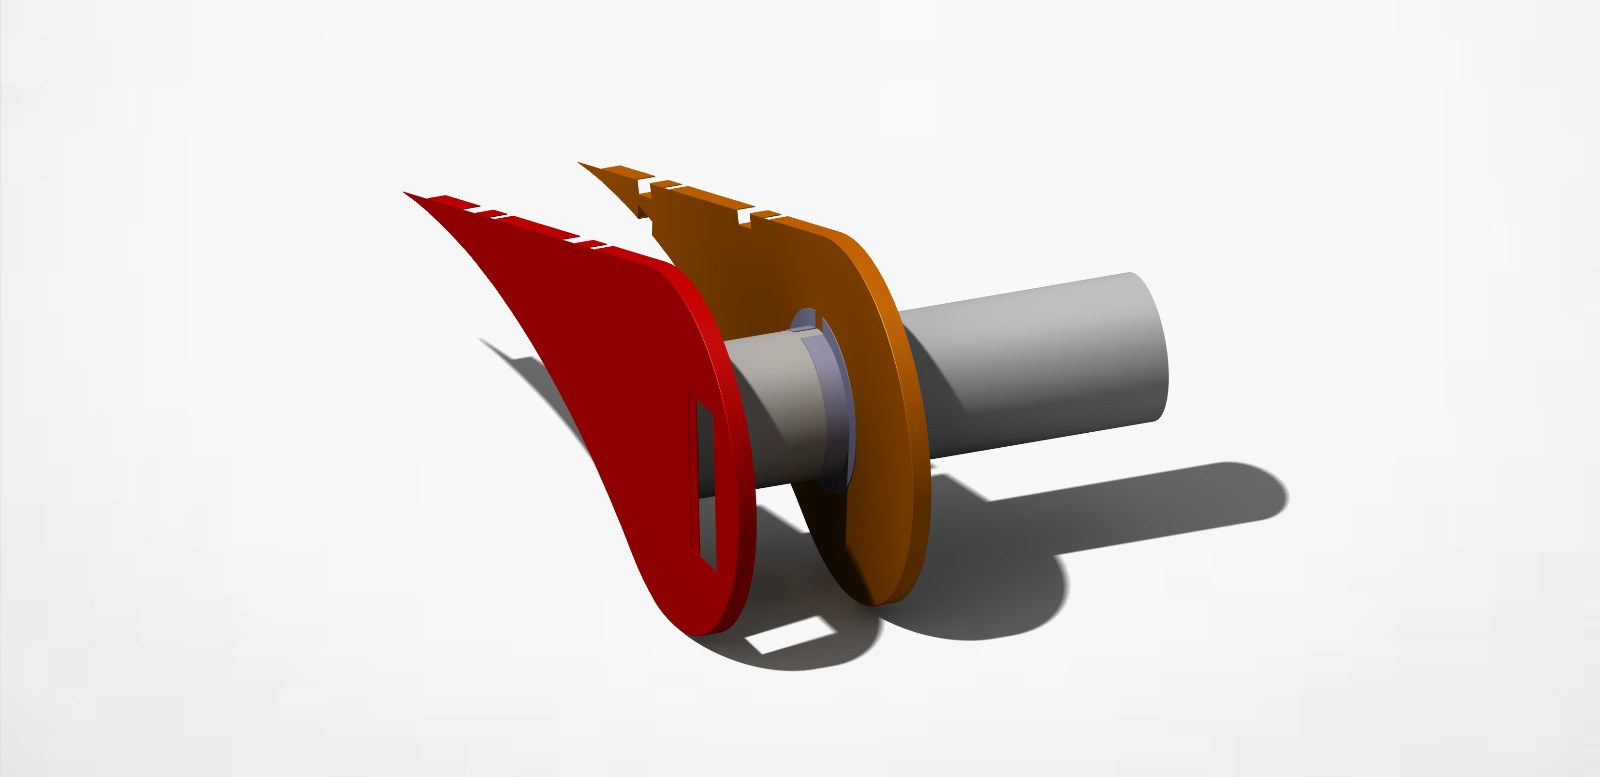
\includegraphics[width=8cm]{Figures/Montaje/5.jpg}}; & \node[lablum=f]{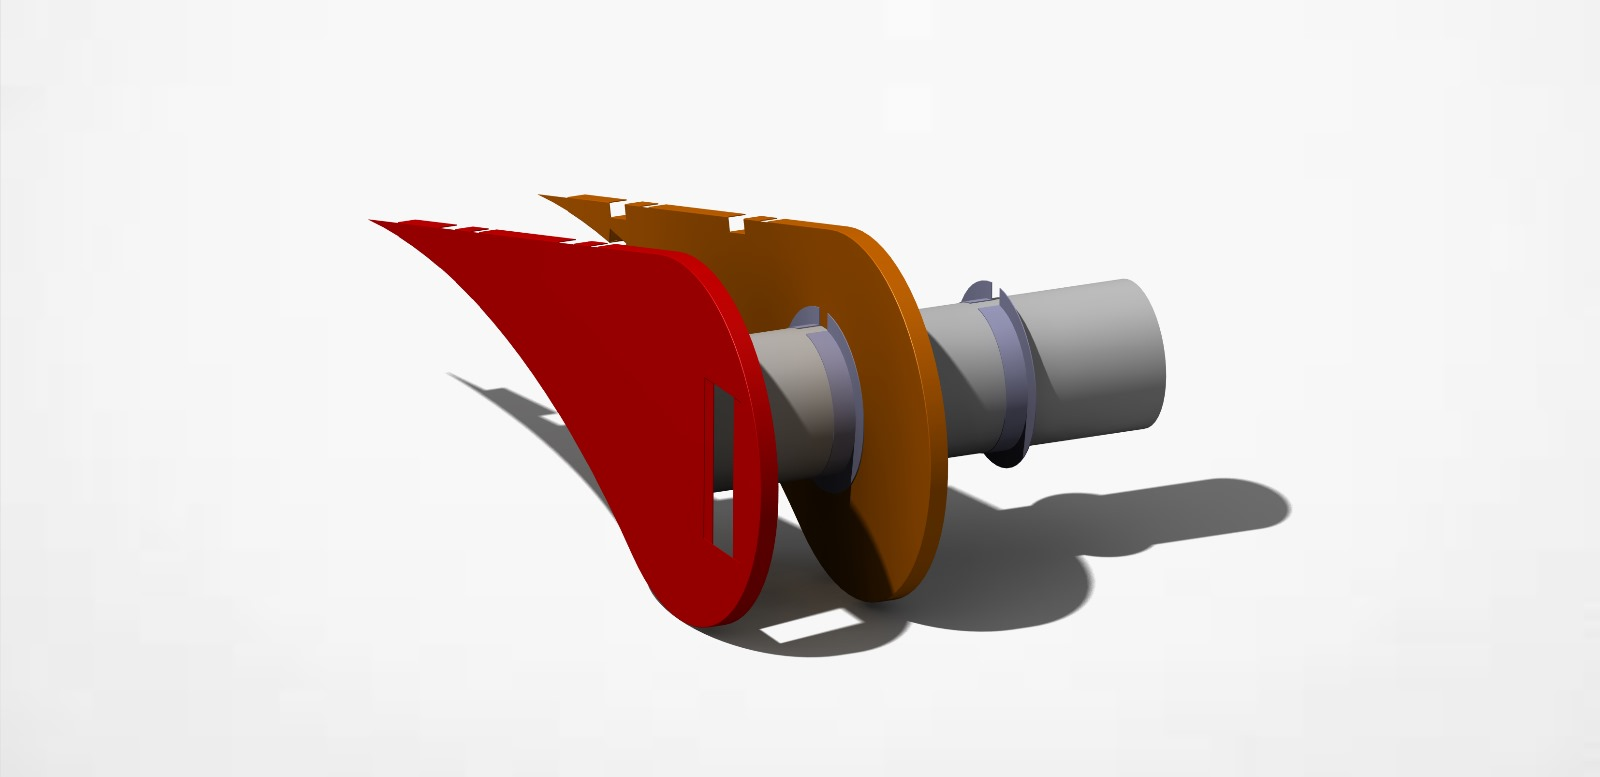
\includegraphics[width=2cm]{Figures/Montaje/6.jpg}}; \\
 };
  \draw[marr] ([xshift=-1mm]img-d.south west) coordinate (aux) 
 -- (img-e.north-|aux);
 \draw[marr] (img-e) -- (img-f);
\end{tikzpicture}
\caption{Quinto Paso. \label{fig:qui}}
\end{figure}
%===============================================================================================================


\subsection{Sexto Paso: Introducción del Sombrerete Delantero}
Análogo a los pasos Segundo y Tercero.

Ver figura \ref{fig:sex}.

%===============================================================================================================
%                                                   SEXTO PASO
%===============================================================================================================
\begin{figure}[!htb]
\centering
\begin{tikzpicture}[lablum/.style 2 args={label=below:#1 #2,name=img-#1},
marr/.style={line width=1mm,-latex}]
 \matrix[column sep=1cm,row sep=5mm] (mat)
 {  \node[lablum=e]{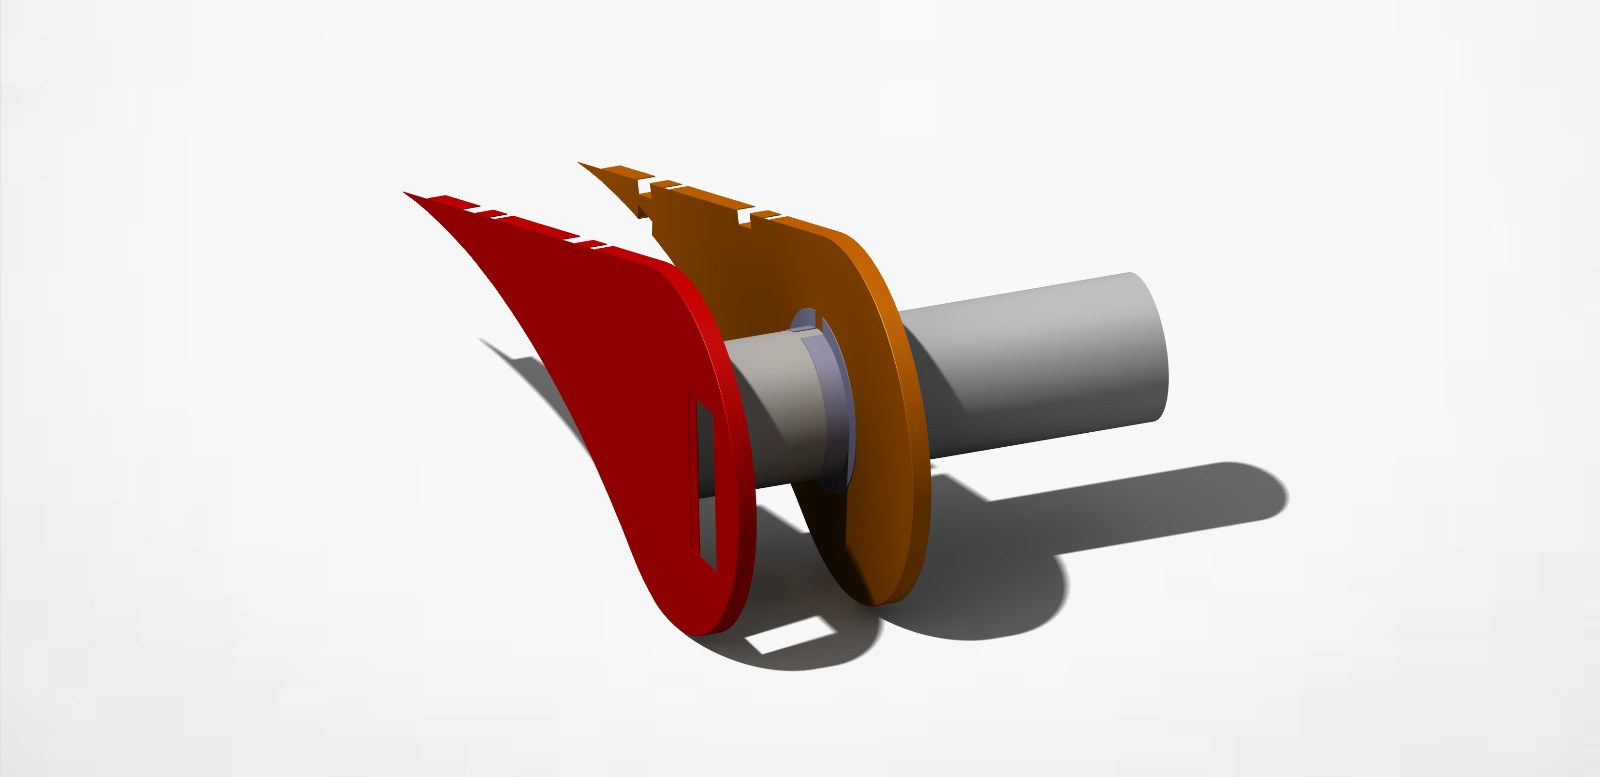
\includegraphics[width=2cm]{Figures/Montaje/5.jpg}}; & \node[lablum=f]{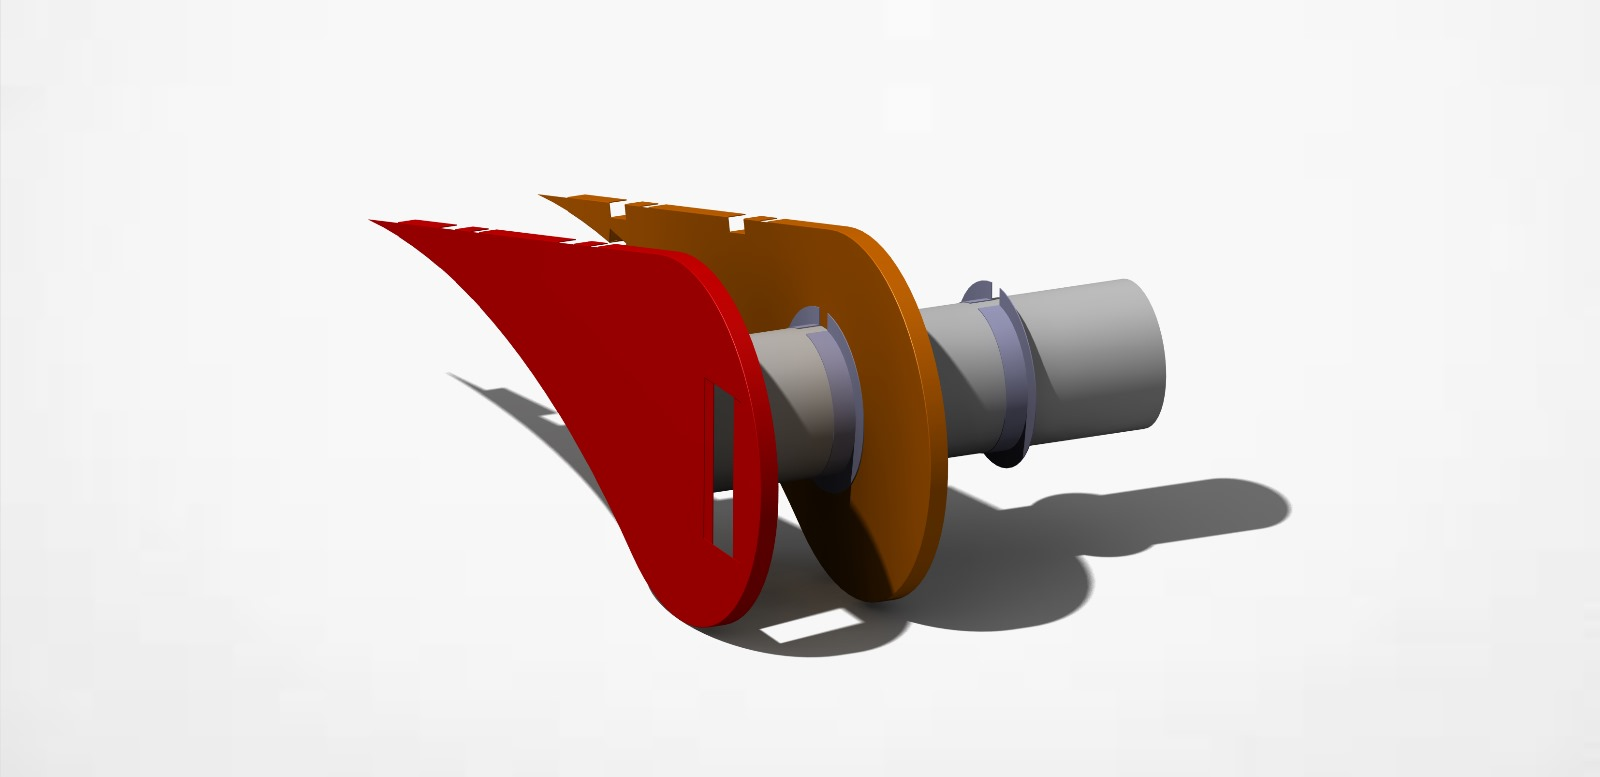
\includegraphics[width=8cm]{Figures/Montaje/6.jpg}}; \\
  & \node[lablum=g]{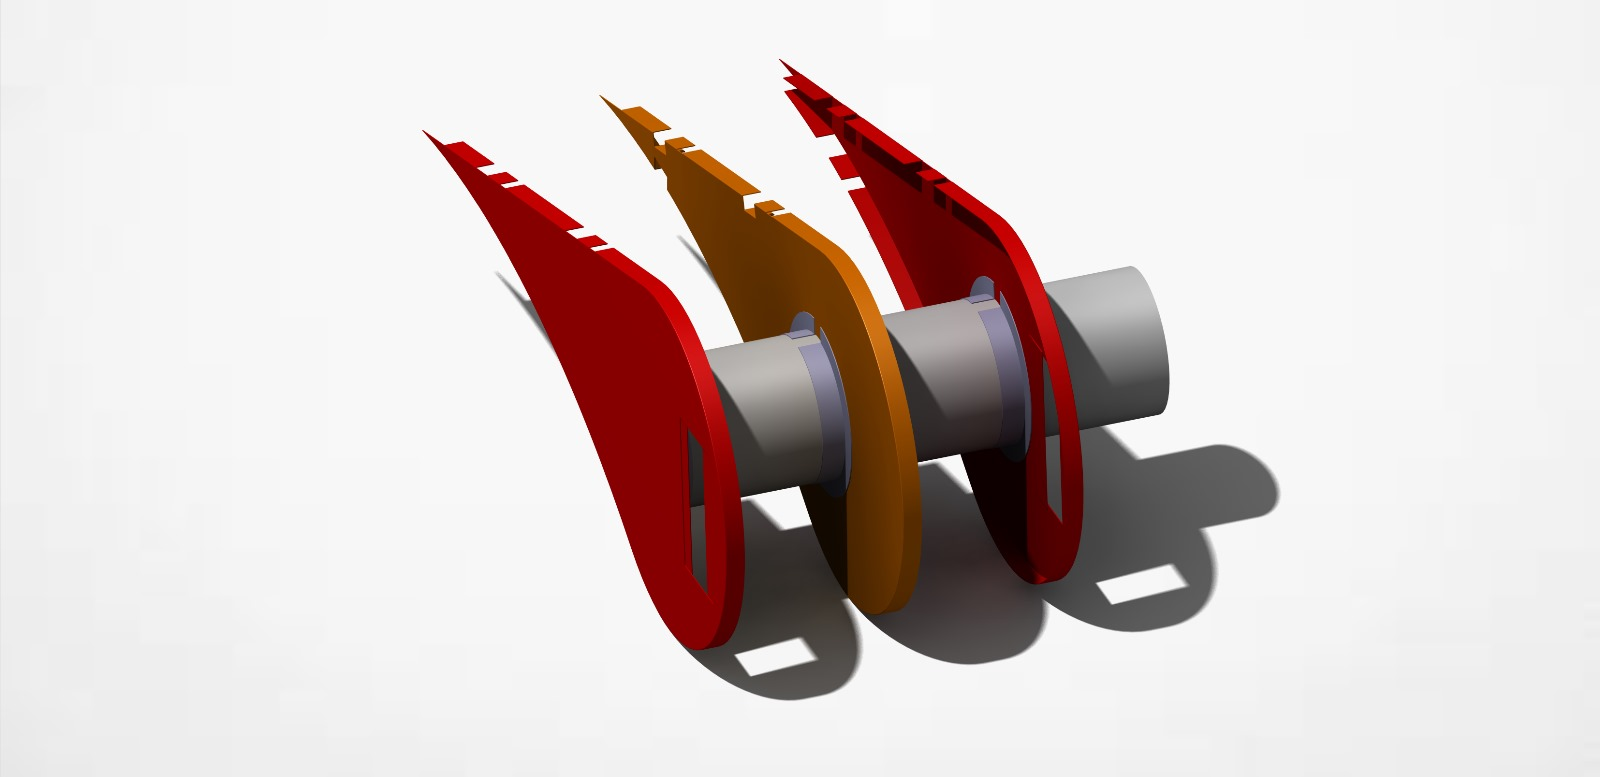
\includegraphics[width=2cm]{Figures/Montaje/7.jpg}};\\ 
 };
 \draw[marr] (img-e) -- (img-f);
  \draw[marr] ([xshift=-1mm]img-f.south east) coordinate (aux) 
 -- (img-g.north-|aux);
\end{tikzpicture}
\caption{Sexto Paso. \label{fig:sex}}
\end{figure}
%===============================================================================================================

\subsection{Séptimo Paso: Unión de la Costilla Delantera}
Se efectúa la unión de la costilla delantera con su sombrerete correspondiente.

Recordemos que la costilla ha de quedar orientada hacia el interior, pero situada al exterior del sombrerete.

Ver figura \ref{fig:sept}.

%===============================================================================================================
%                                                 SÉPTIMO PASO
%===============================================================================================================
\begin{figure}[!htb]
\centering
\begin{tikzpicture}[lablum/.style 2 args={label=below:#1 #2,name=img-#1},
marr/.style={line width=1mm,-latex}]
 \matrix[column sep=1cm,row sep=5mm] (mat)
 {   & \node[lablum=f]{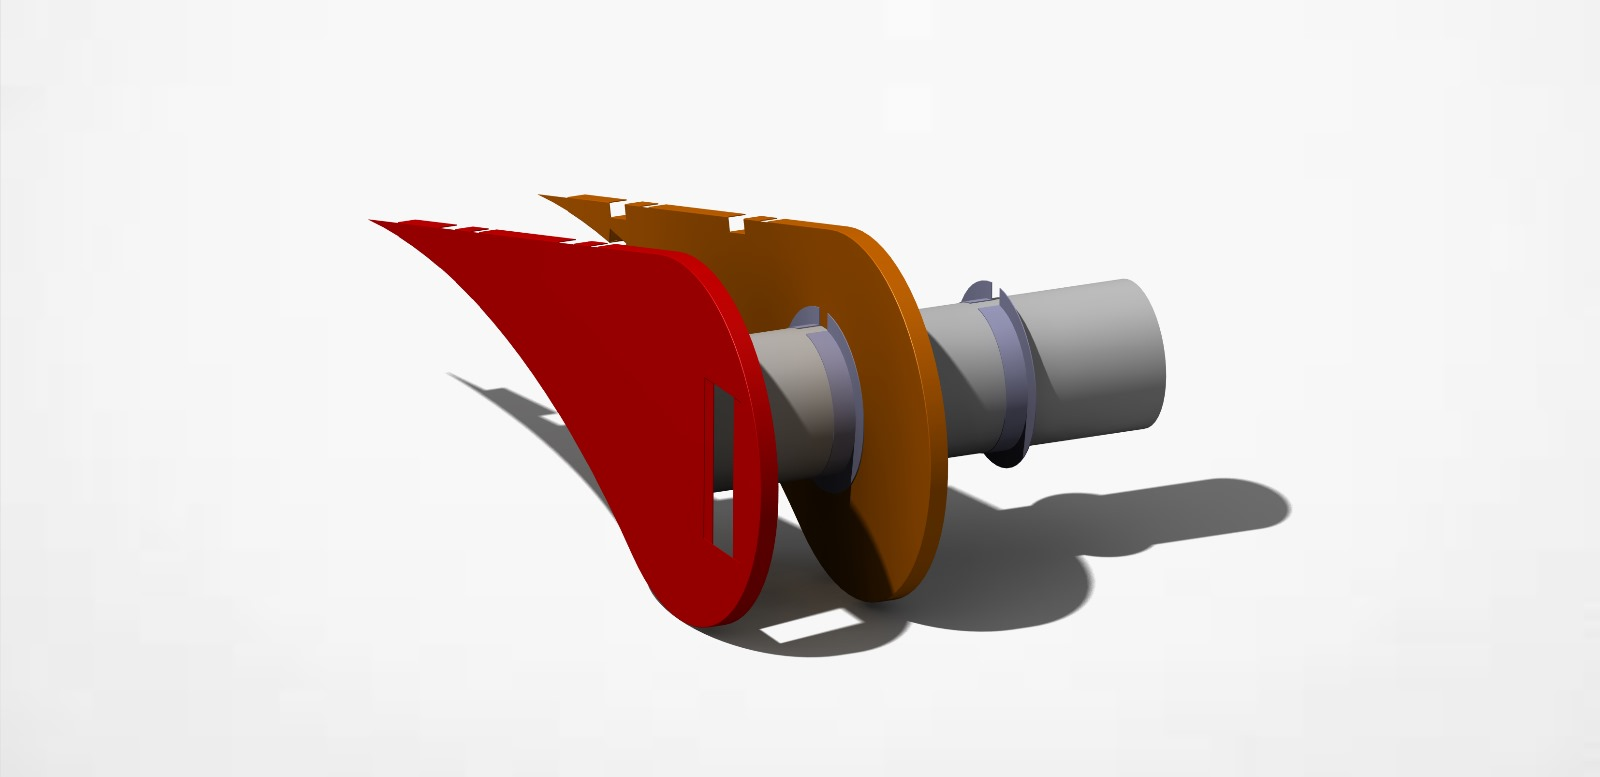
\includegraphics[width=2cm]{Figures/Montaje/6.jpg}}; \\
  \node[lablum=h]{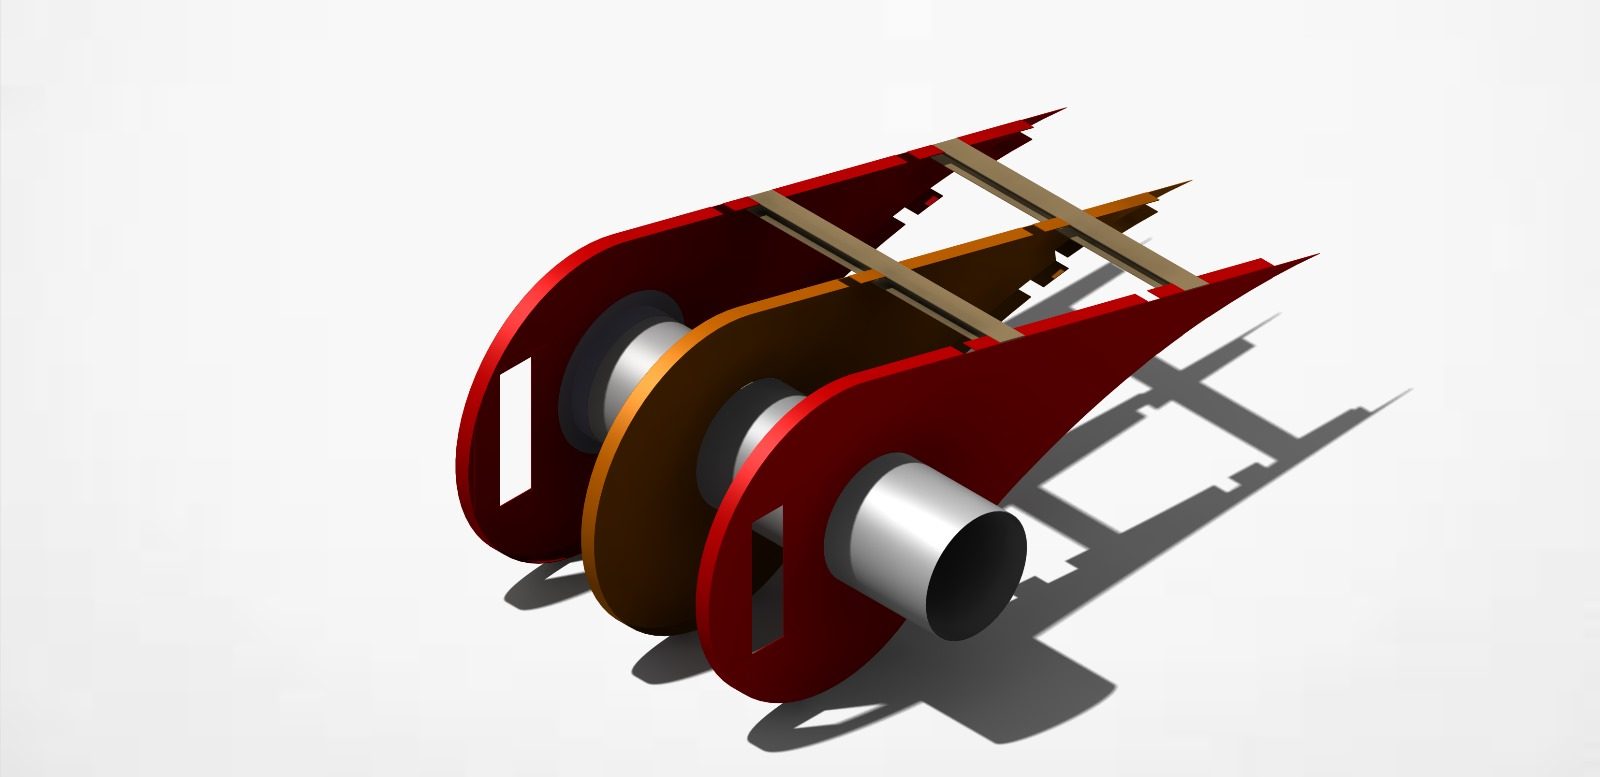
\includegraphics[width=2cm]{Figures/Montaje/8.jpg}}; & \node[lablum=g]{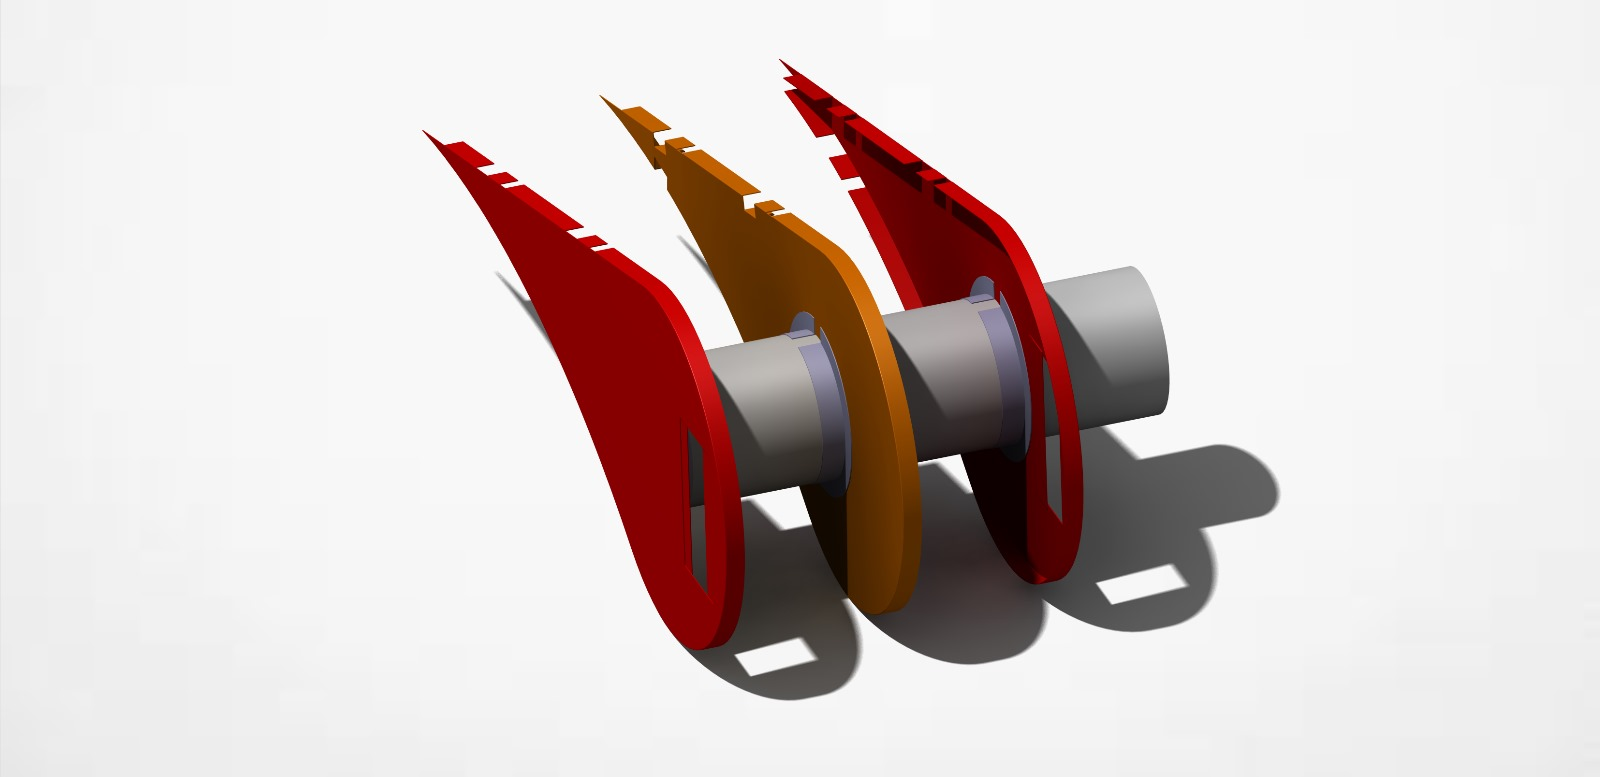
\includegraphics[width=8cm]{Figures/Montaje/7.jpg}}; \\
 };
\draw[marr] ([xshift=-1mm]img-f.south east) coordinate (aux) 
 -- (img-g.north-|aux);
 \draw[marr] (img-g) -- (img-h);
\end{tikzpicture}
\caption{Séptimo Paso. \label{fig:sept}}
\end{figure}
%===============================================================================================================


\subsection{Octavo y Noveno Pasos: Larguerillos}
Introducimos cuatro larguerillos, dos superiores (Paso Octavo) y dos inferiores (Paso Noveno), de 398 [mm] en la estructura. Se colocarán sobre las ranuras de las costillas, y se unirán a ellas mediante soldadura por puntos.

Los larguerillos son necesarios ya que ayudan a mantener la integridad de la estructura.

Ver figuras \ref{fig:oct} y \ref{fig:nov}.

%===============================================================================================================
%                                                   OCTAVO PASO
%===============================================================================================================


\begin{figure}[!htb]
\centering
\begin{tikzpicture}[lablum/.style 2 args={label=below:#1 #2,name=img-#1},
marr/.style={line width=1mm,-latex}]
 \matrix[column sep=1cm,row sep=5mm] (mat)
 {   
  \node[lablum=h]{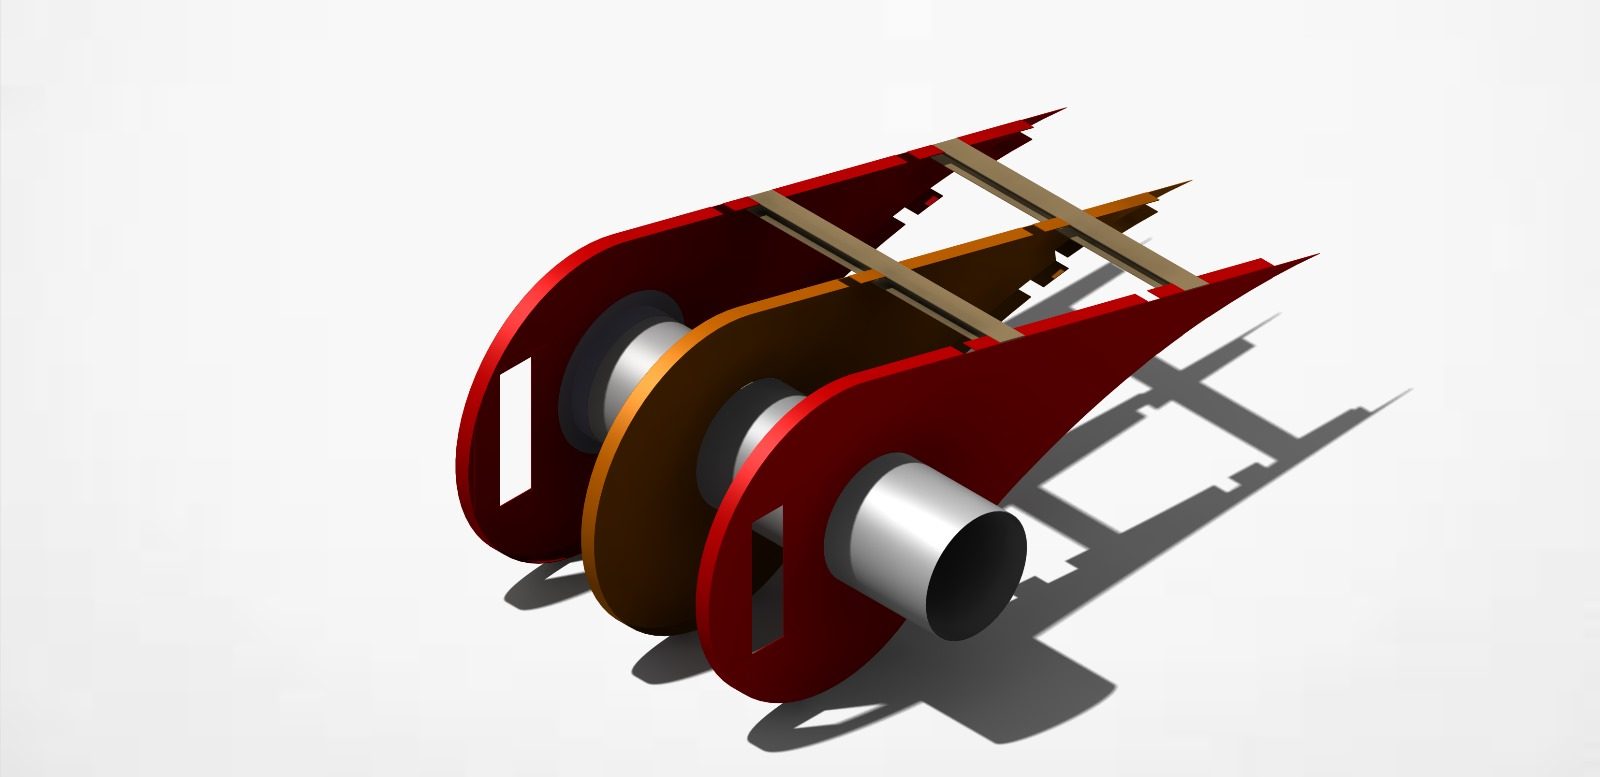
\includegraphics[width=8cm]{Figures/Montaje/8.jpg}}; & \node[lablum=g]{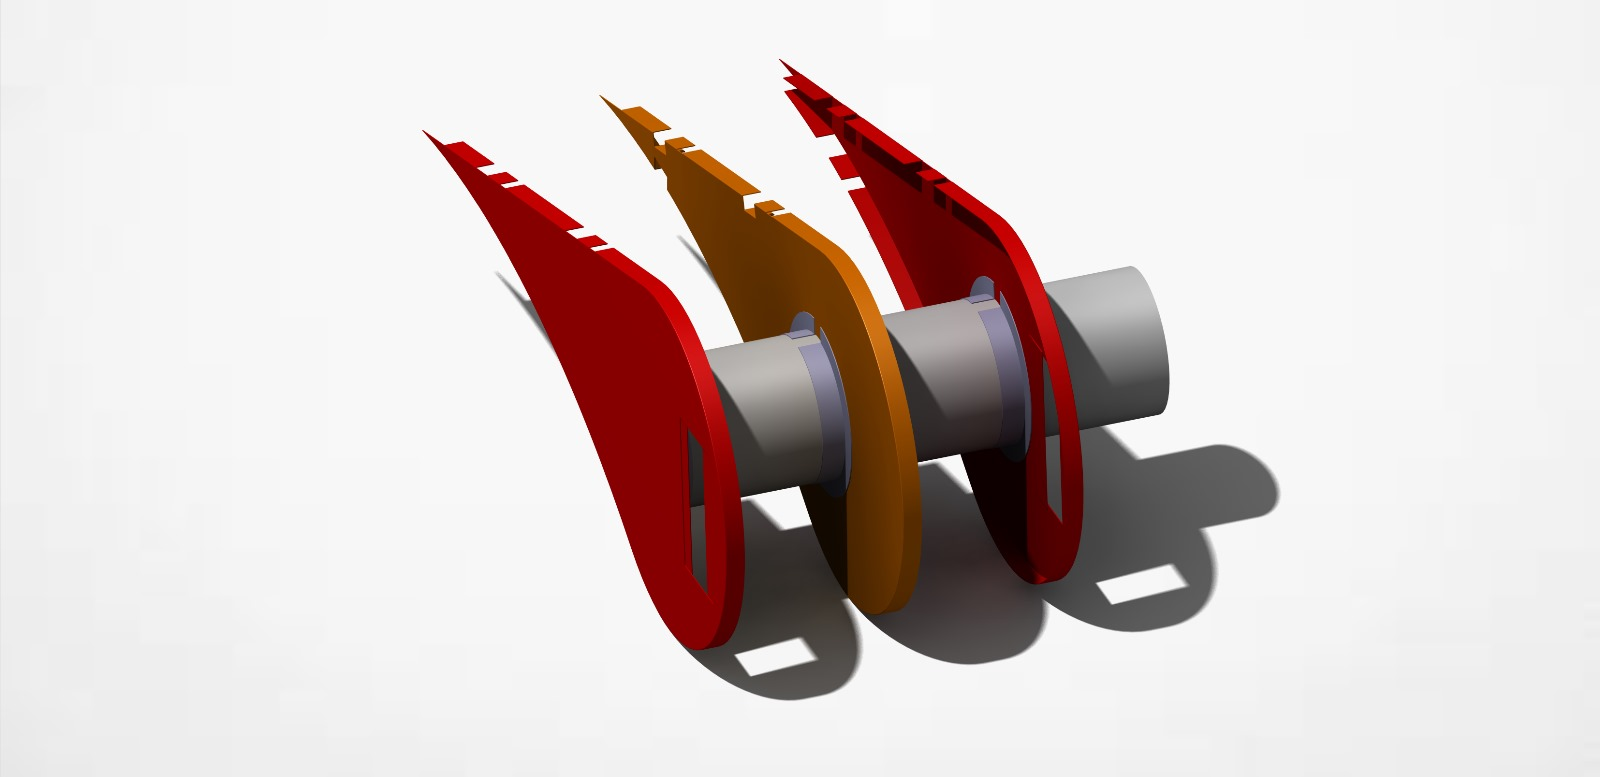
\includegraphics[width=2cm]{Figures/Montaje/7.jpg}};\\  \node[lablum=i]{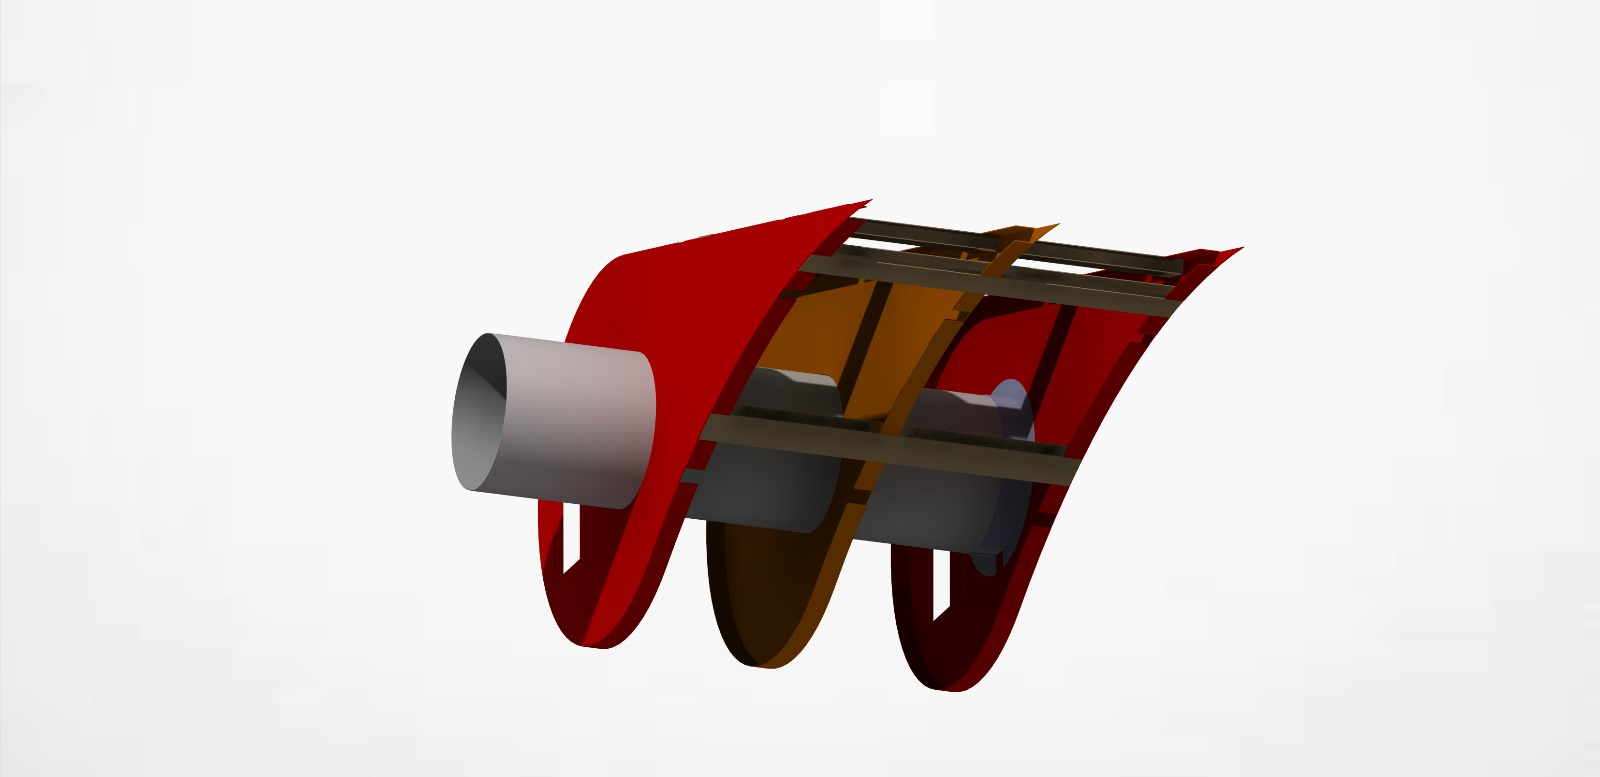
\includegraphics[width=2cm]{Figures/Montaje/9.jpg}}; \\
 };
 \draw[marr] (img-g) -- (img-h);
  \draw[marr] ([xshift=1mm]img-h.south west) coordinate (aux) 
 -- (img-i.north-|aux);
\end{tikzpicture}
\caption{Octavo Paso. \label{fig:oct}}
\end{figure}
%===============================================================================================================

%===============================================================================================================
%                                                   NOVENO PASO
%===============================================================================================================
\begin{figure}[!htb]
\centering
\begin{tikzpicture}[lablum/.style 2 args={label=below:#1 #2,name=img-#1},
marr/.style={line width=1mm,-latex}]
 \matrix[column sep=1cm,row sep=5mm] (mat)
 {   
  \node[lablum=h]{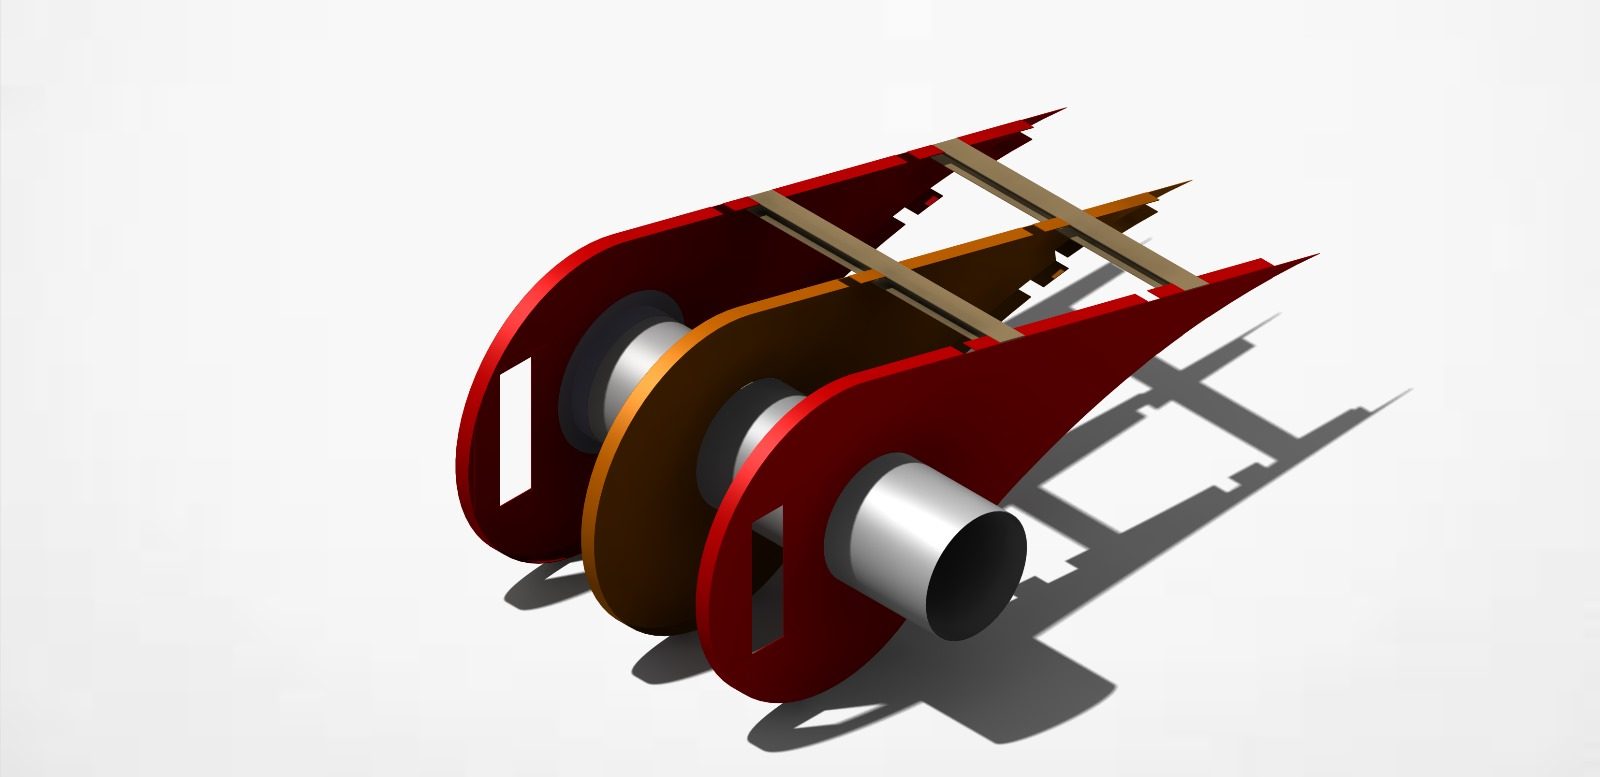
\includegraphics[width=2cm]{Figures/Montaje/8.jpg}}; & \\  \node[lablum=i]{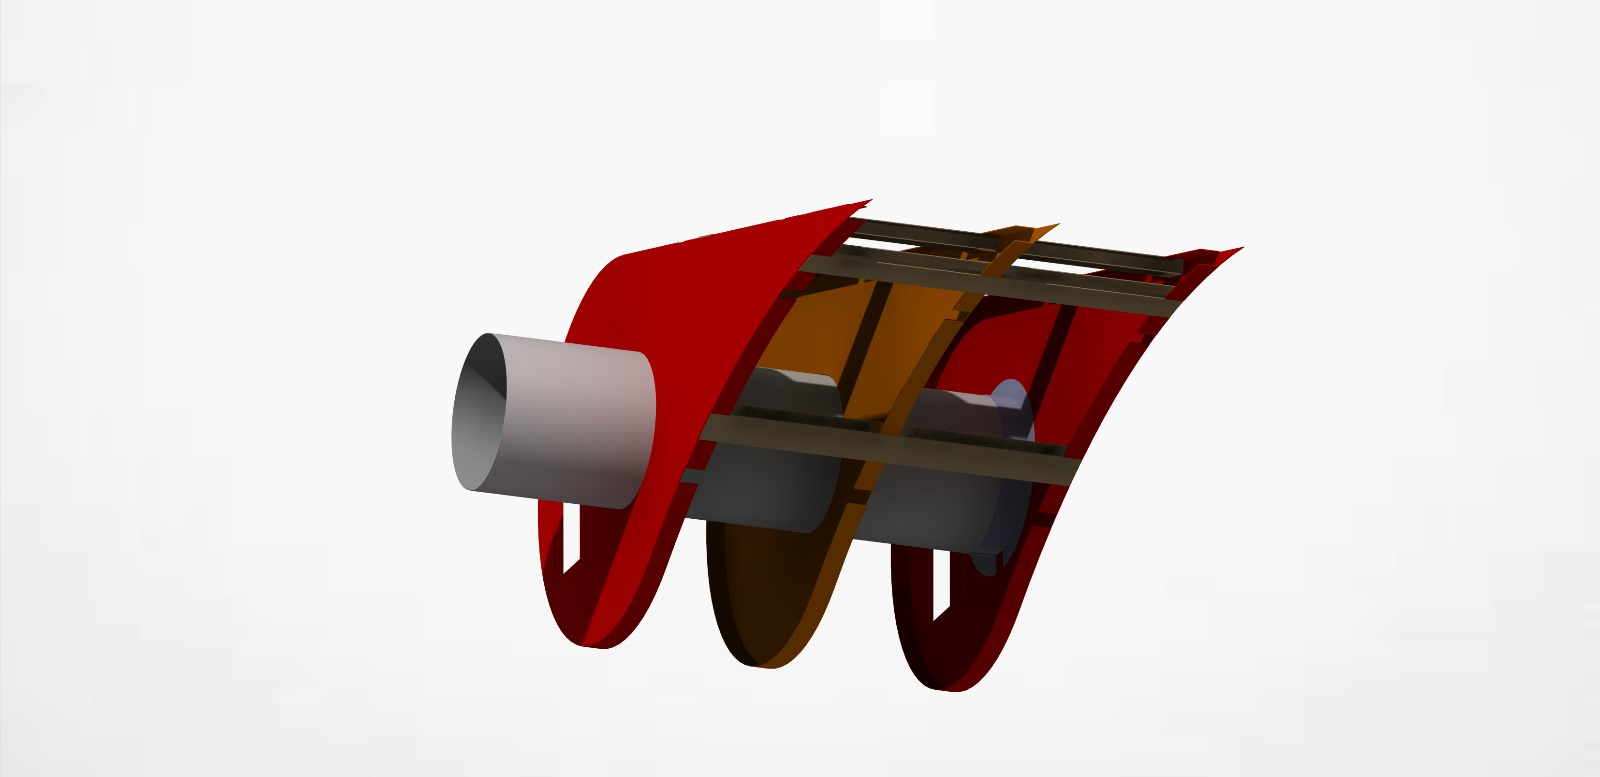
\includegraphics[width=8cm]{Figures/Montaje/9.jpg}}; & \node[lablum=j]{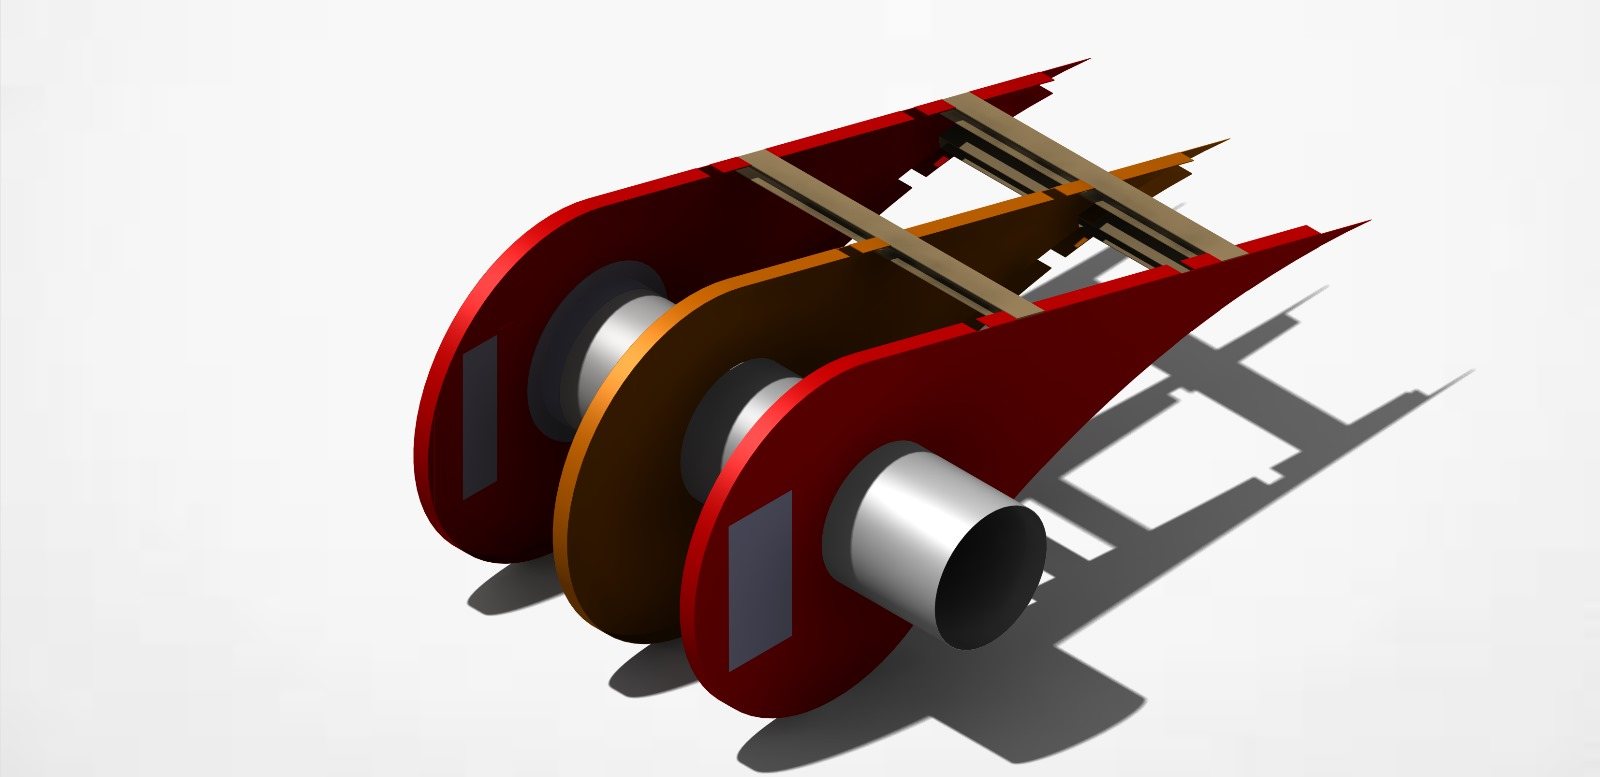
\includegraphics[width=2cm]{Figures/Montaje/10.jpg}}; \\
 };
\draw[marr] ([xshift=1mm]img-h.south west) coordinate (aux) 
 -- (img-i.north-|aux);
 \draw[marr] (img-i) -- (img-j);
\end{tikzpicture}
\caption{Noveno Paso. \label{fig:nov}}
\end{figure}
%===============================================================================================================
\pagebreak
\subsection{Décimo Paso: Tapa de Acceso}
Este proceso se realizará tanto para la costilla trasera como para la trasera.

La tapa de acceso, de dimensiones 180$\times$90, se unirá a la costilla mediante un remachado visible con cabeza universal, que se podrá quitar para acceder a la estructura interior. La estructura ha de estar levemente hundida para que, cuando se remache, quede lisa, y no afecta al comportamiento aerodinámico.

Con un granete se marca la pieza y, posteriormente, se taladra. Se pinza para sujetar los remaches en su lugar, mientras se aplica la fuerza para fijarlos. Una vez remachado, se efectúa el avellanado.

Ver figura \ref{fig:dec}.

%===============================================================================================================
%                                                   DÉCIMO PASO
%===============================================================================================================
\begin{figure}[!htb]
\centering
\begin{tikzpicture}[lablum/.style 2 args={label=below:#1 #2,name=img-#1},
marr/.style={line width=1mm,-latex}]
 \matrix[column sep=1cm,row sep=5mm] (mat)
 { \node[lablum=i]{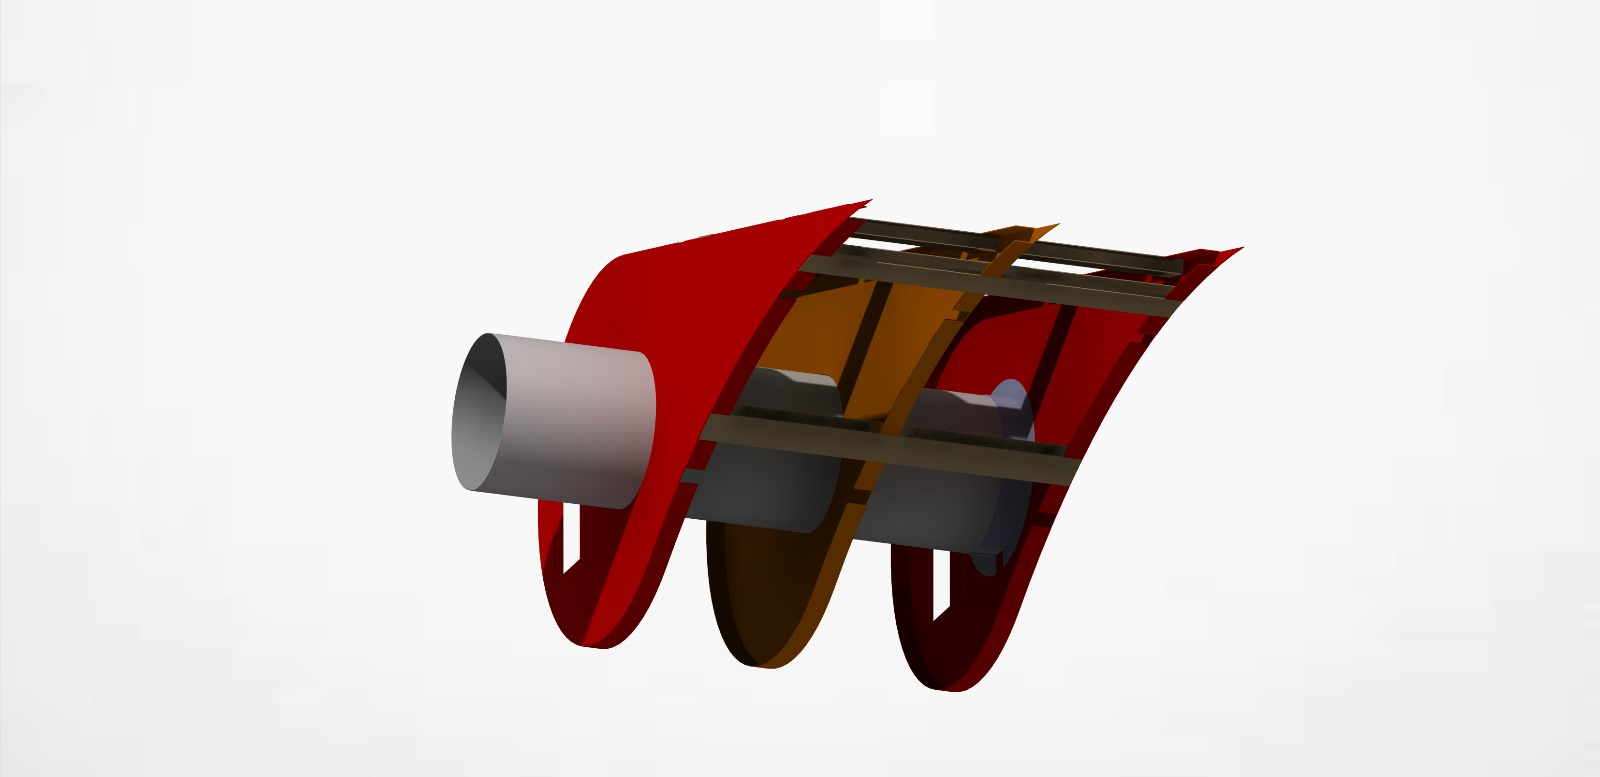
\includegraphics[width=2cm]{Figures/Montaje/9.jpg}}; & \node[lablum=j]{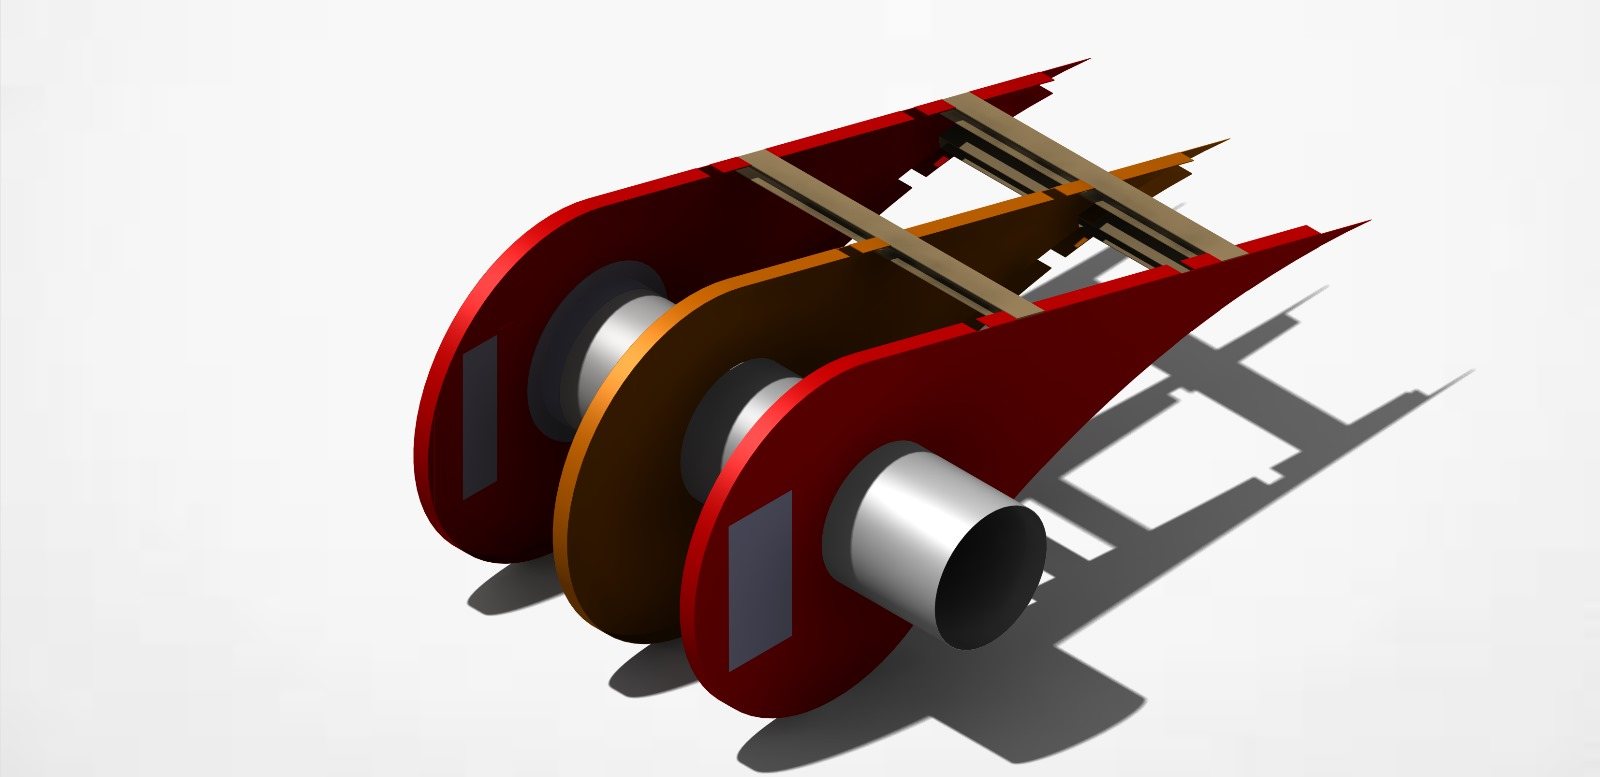
\includegraphics[width=8cm]{Figures/Montaje/10.jpg}}; \\ 
 & \node[lablum=k]{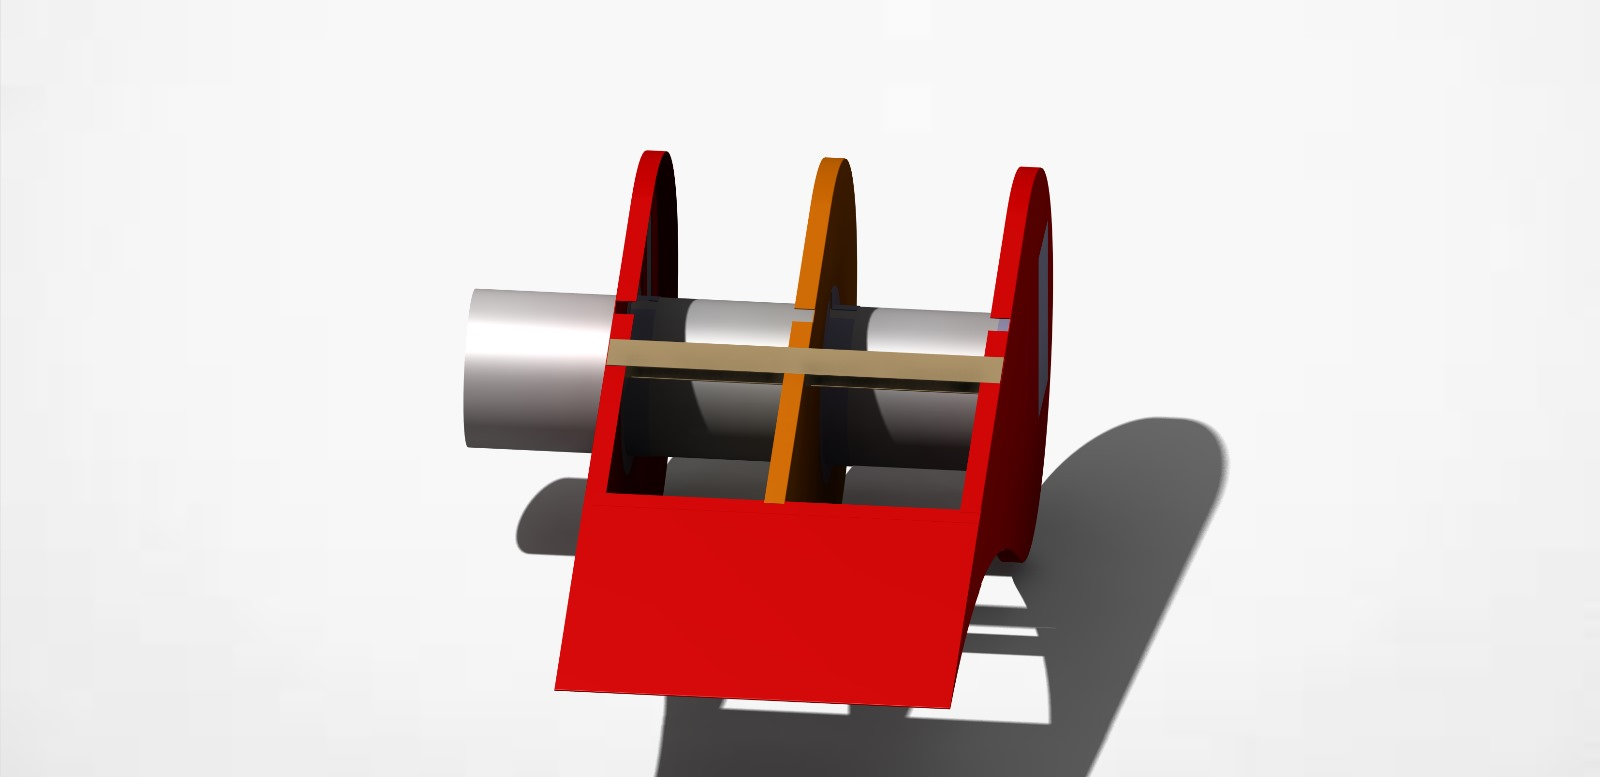
\includegraphics[width=2cm]{Figures/Montaje/11.jpg}}; \\
 };
 \draw[marr] (img-i) -- (img-j);
  \draw[marr] ([xshift=-1mm]img-j.south east) coordinate (aux) 
 -- (img-k.north-|aux);
\end{tikzpicture}
\caption{Décimo Paso. \label{fig:dec}}
\end{figure}
%===============================================================================================================

\pagebreak
\subsection{Undécimo Paso: Revestimiento del Borde de Salida}
Colocamos el primer revestimiento, que ha sido moldeado para que adquiera la forma del borde de salida, y que, además, cuenta con los extremos doblados para que se introduzca a las ranuras de la costilla.

Como la soldadura no es conveniente aquí (produce una deformación indeseada), el proceso se realizará mediante remachado ciego, con posterior avellanado, a fin de evitar que la cabeza sobresalga de la superficie. 

El remachado ha sido explicado en detalle en el paso anterior.

Ver figura \ref{fig:und}.

%===============================================================================================================
%                                                  11º PASO
%===============================================================================================================
\begin{figure}[!htb]
\centering
\begin{tikzpicture}[lablum/.style 2 args={label=below:#1 #2,name=img-#1},
marr/.style={line width=1mm,-latex}]
 \matrix[column sep=1cm,row sep=5mm] (mat)
 { & \node[lablum=j]{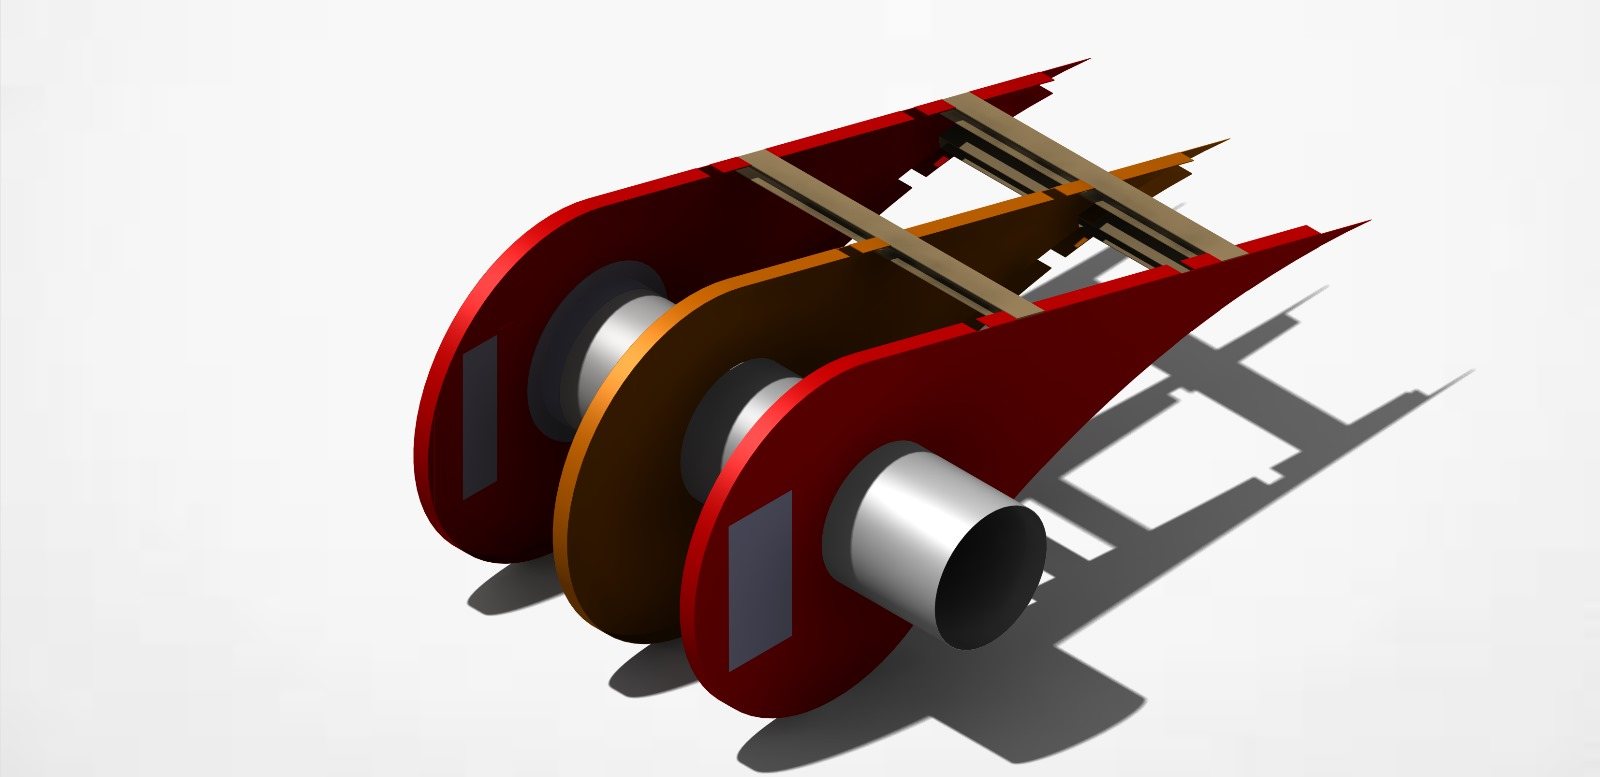
\includegraphics[width=2cm]{Figures/Montaje/10.jpg}}; \\ 
\node[lablum=l]{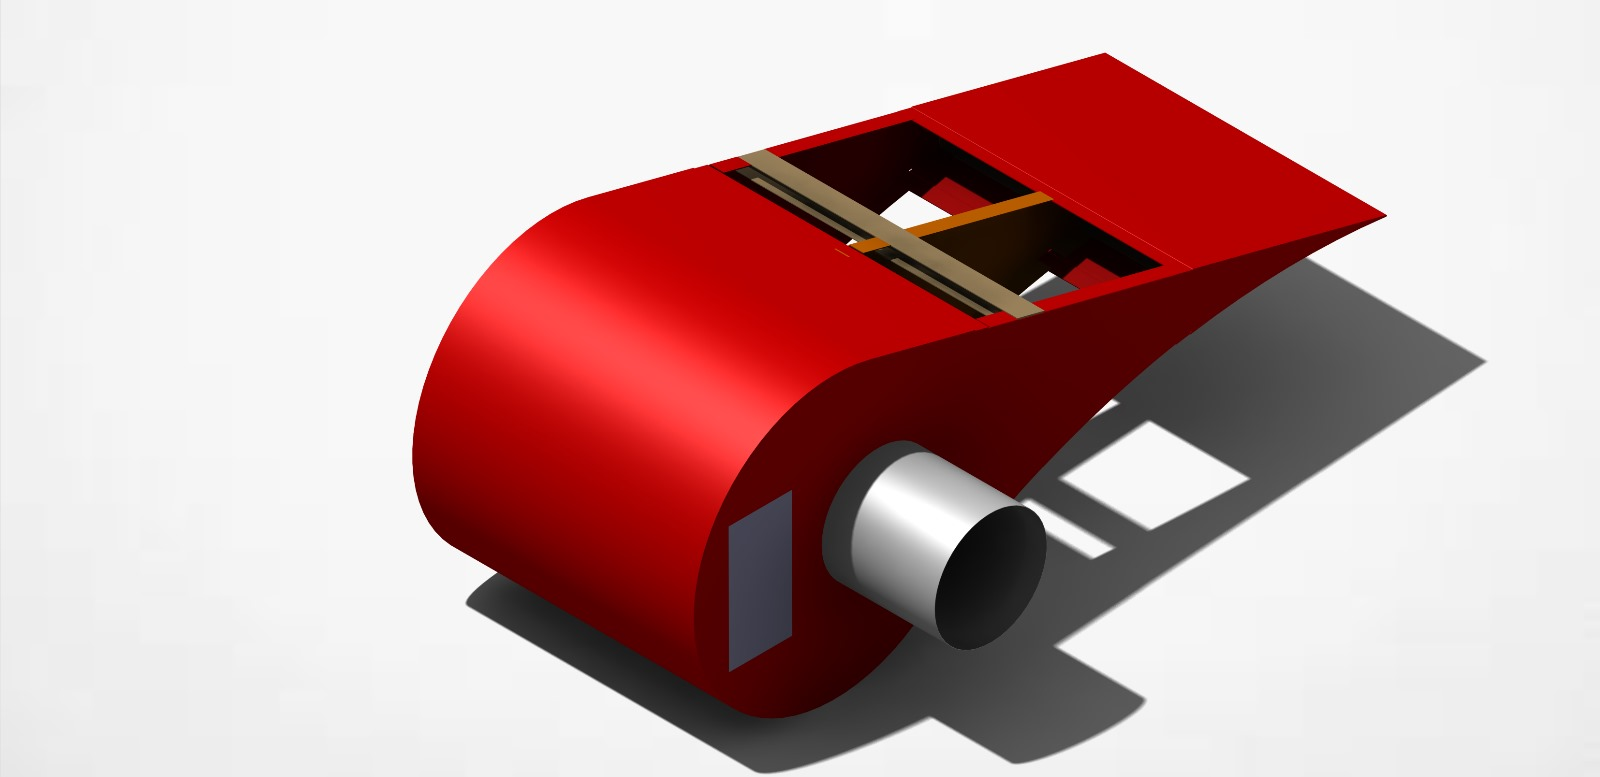
\includegraphics[width=2cm]{Figures/Montaje/12.jpg}}; & \node[lablum=k]{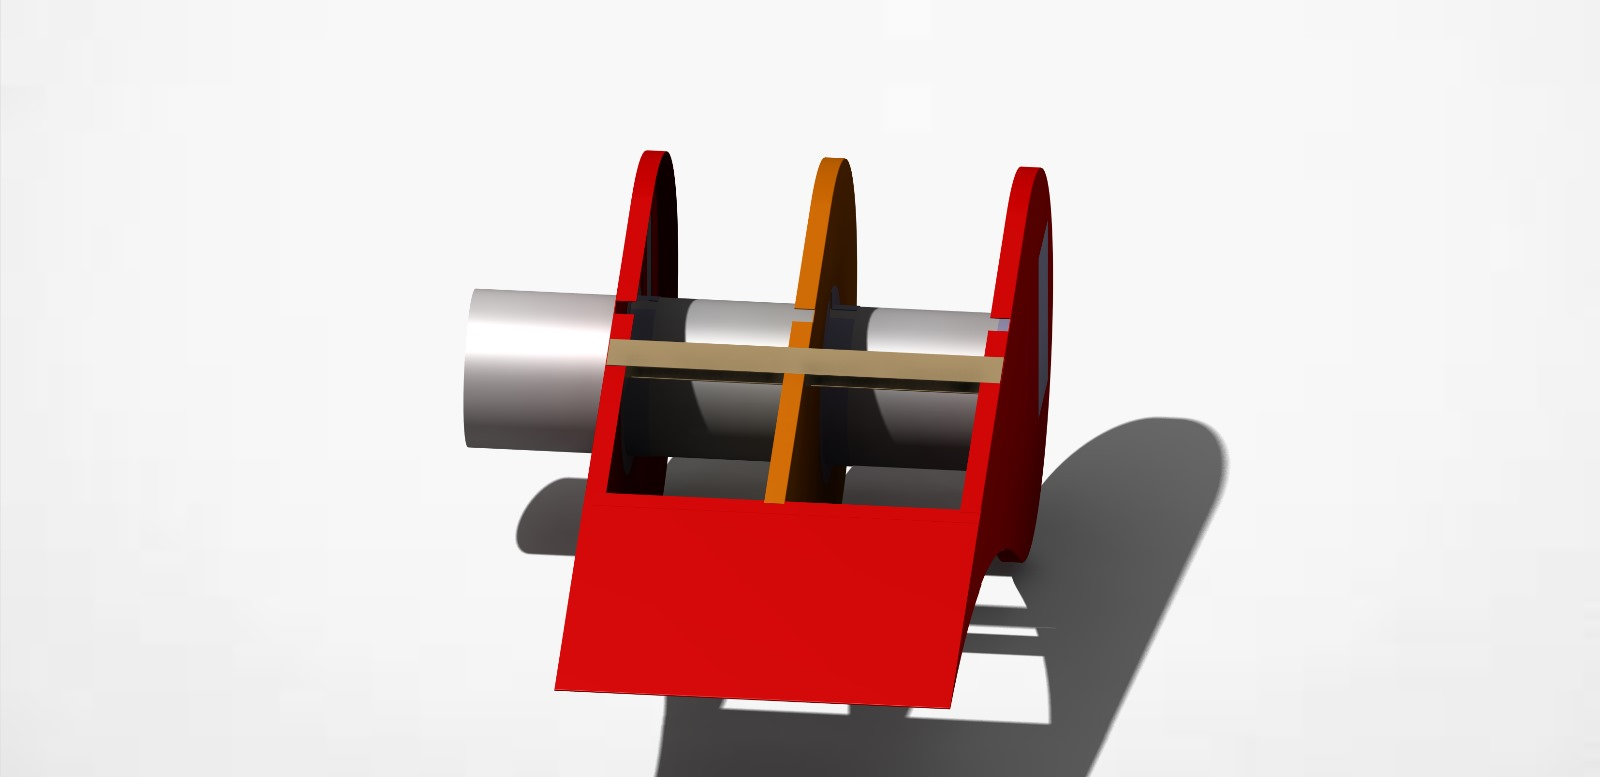
\includegraphics[width=8cm]{Figures/Montaje/11.jpg}}; \\
 };
\draw[marr] ([xshift=-1mm]img-j.south east) coordinate (aux) 
 -- (img-k.north-|aux);
  \draw[marr] (img-k) -- (img-l);
\end{tikzpicture}
\caption{Undécimo Paso. \label{fig:und}}
\end{figure}
%===============================================================================================================

\pagebreak
\subsection{Duodécimo Paso: Revestimiento del Borde de Ataque}
Análogo al paso anterior. Colocamos el revestimiento, que ha sido moldeado con forma del borde de ataque, siguiendo el procedimiento descrito en el paso anterior.

Ver figura \ref{fig:duo}.

%===============================================================================================================
%                                                   12º PASO
%===============================================================================================================
\begin{figure}[!htb]
\centering
\begin{tikzpicture}[lablum/.style 2 args={label=below:#1 #2,name=img-#1},
marr/.style={line width=1mm,-latex}]
 \matrix[column sep=1cm,row sep=5mm] (mat)
 { \node[lablum=l]{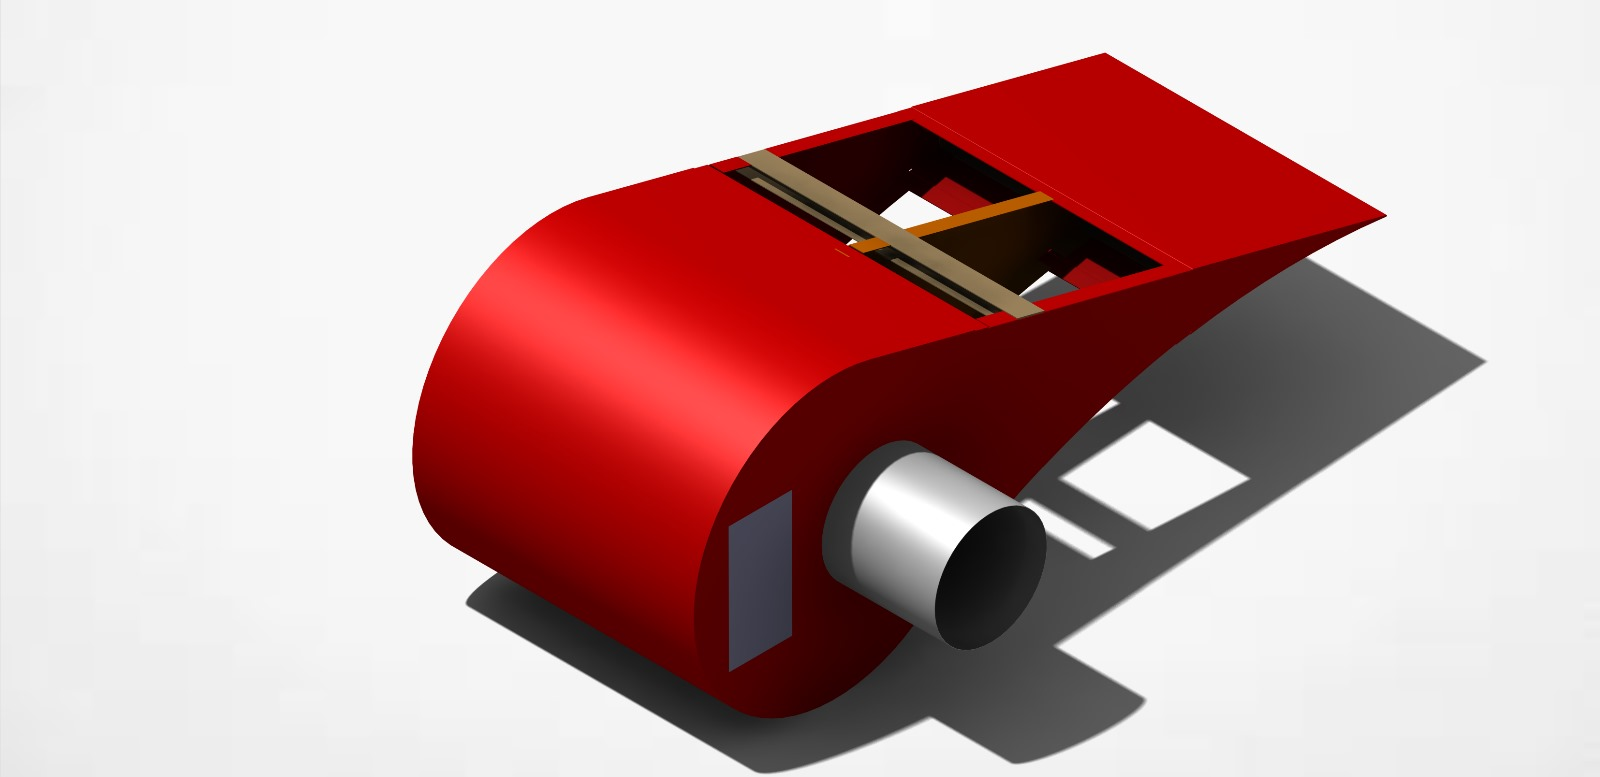
\includegraphics[width=8cm]{Figures/Montaje/12.jpg}}; & \node[lablum=k]{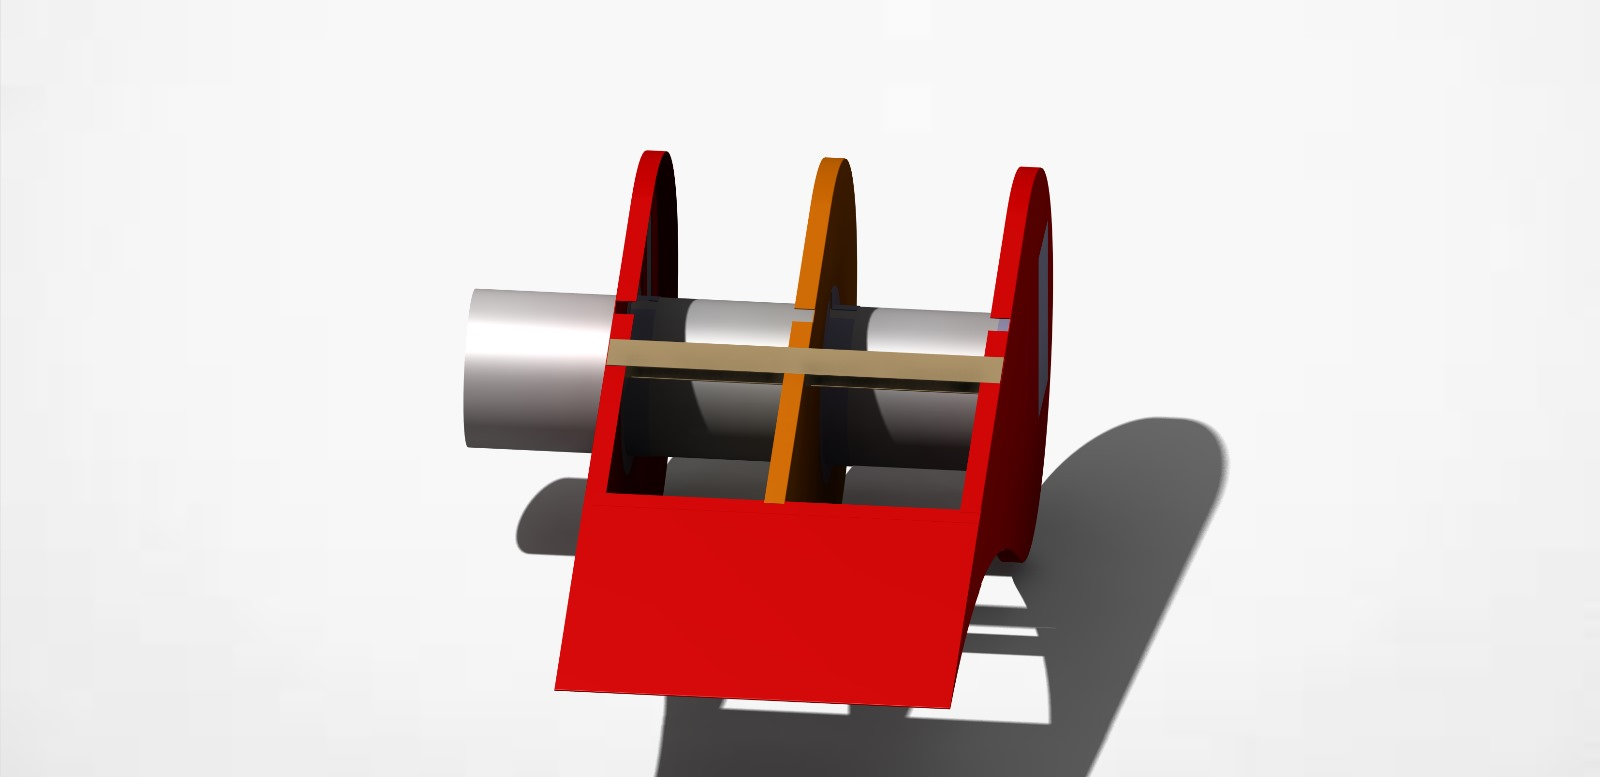
\includegraphics[width=2cm]{Figures/Montaje/11.jpg}}; \\
 \node[lablum=m]{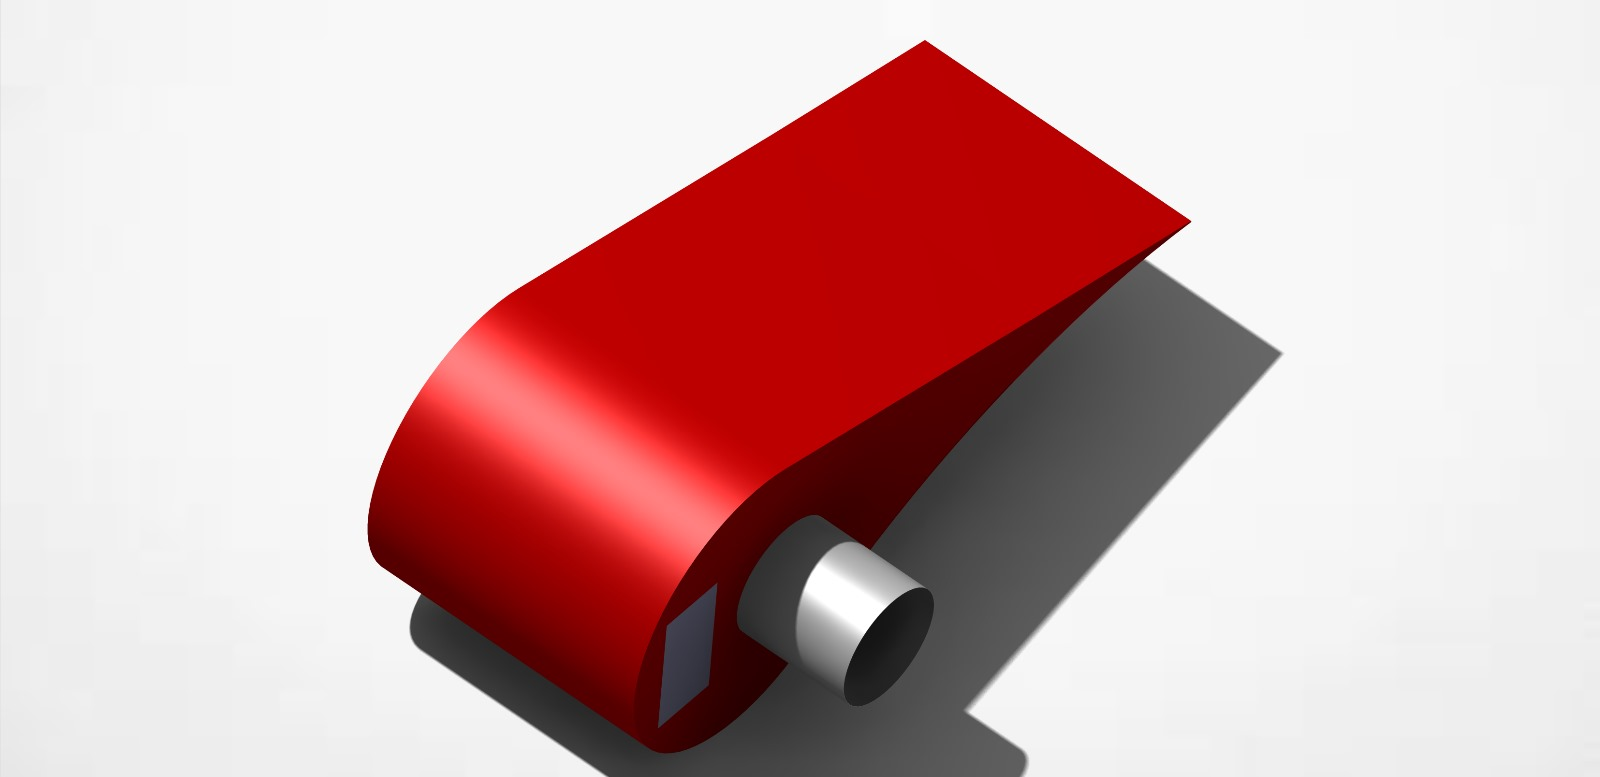
\includegraphics[width=2cm]{Figures/Montaje/13.jpg}}; &  \\
 };
\draw[marr] (img-k) -- (img-l);
\draw[marr] ([xshift=1mm]img-l.south west) coordinate (aux) 
 -- (img-m.north-|aux);
\end{tikzpicture}
\caption{Duodécimo Paso.\label{fig:duo}}
\end{figure}
%===============================================================================================================

\pagebreak
\subsection{Decimotercer Paso: Revestimiento del Extradós}
Se efectúa un remachado de caña maciza con avellanado posterior. Como el revestimiento del intradós aún no ha sido colocado, tenemos acceso en sendas partes, por lo que podemos realizar un remachado no ciego.

Ver figura \ref{fig:dete}.

%===============================================================================================================
%                                                   13º PASO
%===============================================================================================================
\begin{figure}[!htb]
\centering
\begin{tikzpicture}[lablum/.style 2 args={label=below:#1 #2,name=img-#1},
marr/.style={line width=1mm,-latex}]
 \matrix[column sep=1cm,row sep=5mm] (mat)
 { \node[lablum=l]{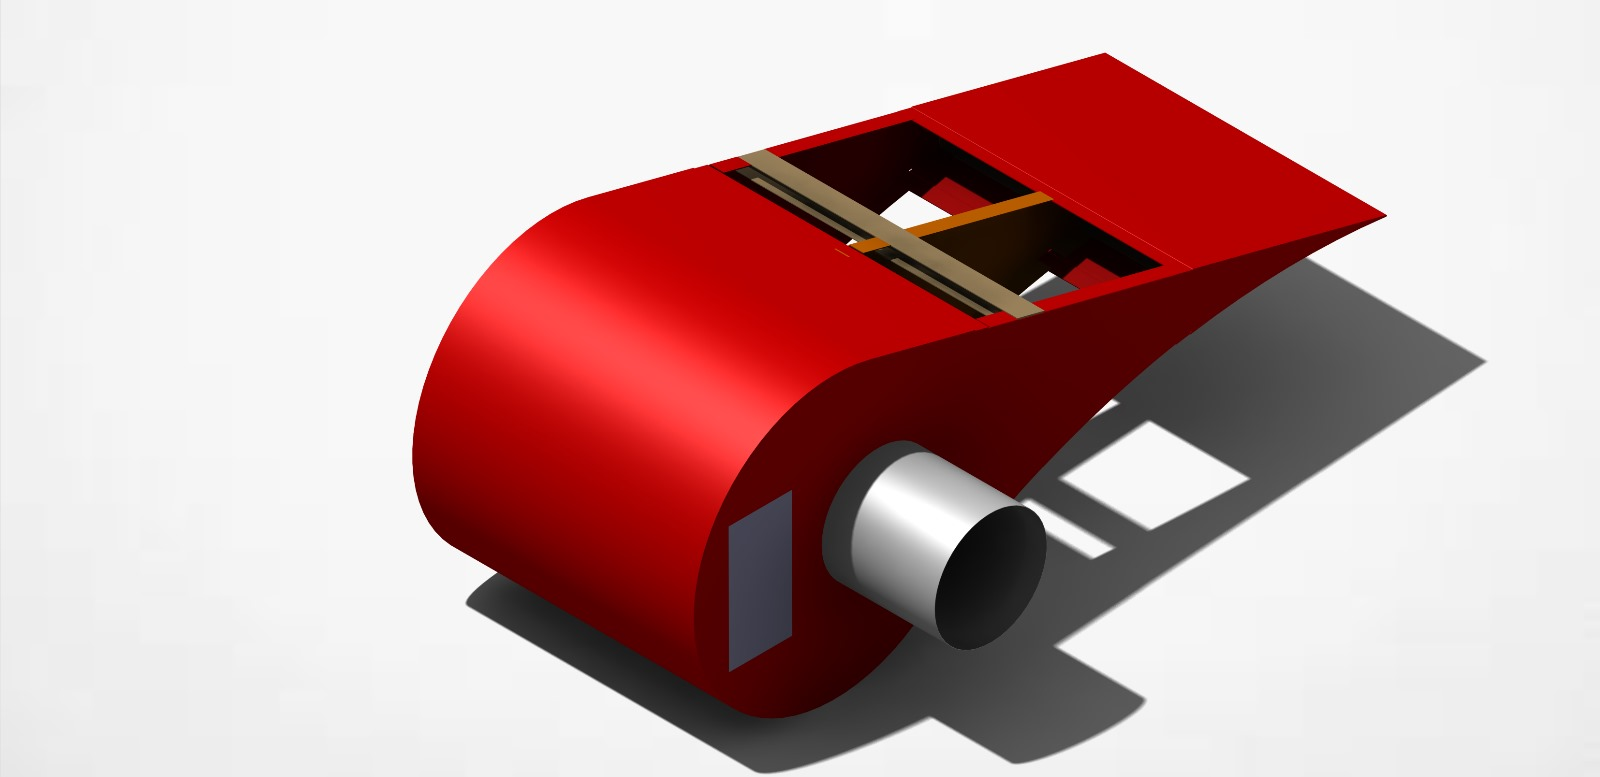
\includegraphics[width=2cm]{Figures/Montaje/12.jpg}}; &  \\
 \node[lablum=m]{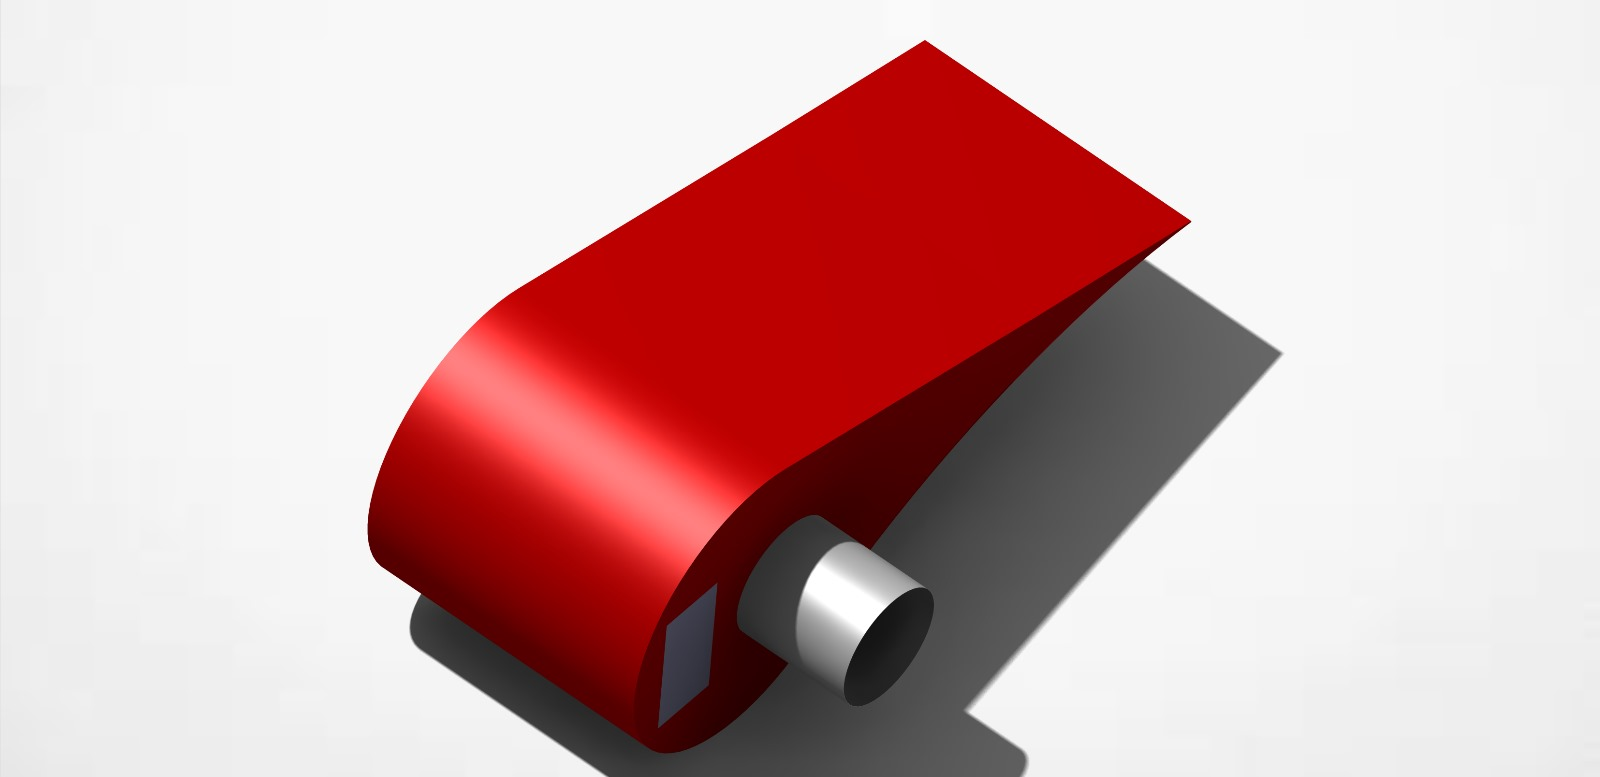
\includegraphics[width=8cm]{Figures/Montaje/13.jpg}}; & \node[lablum=n]{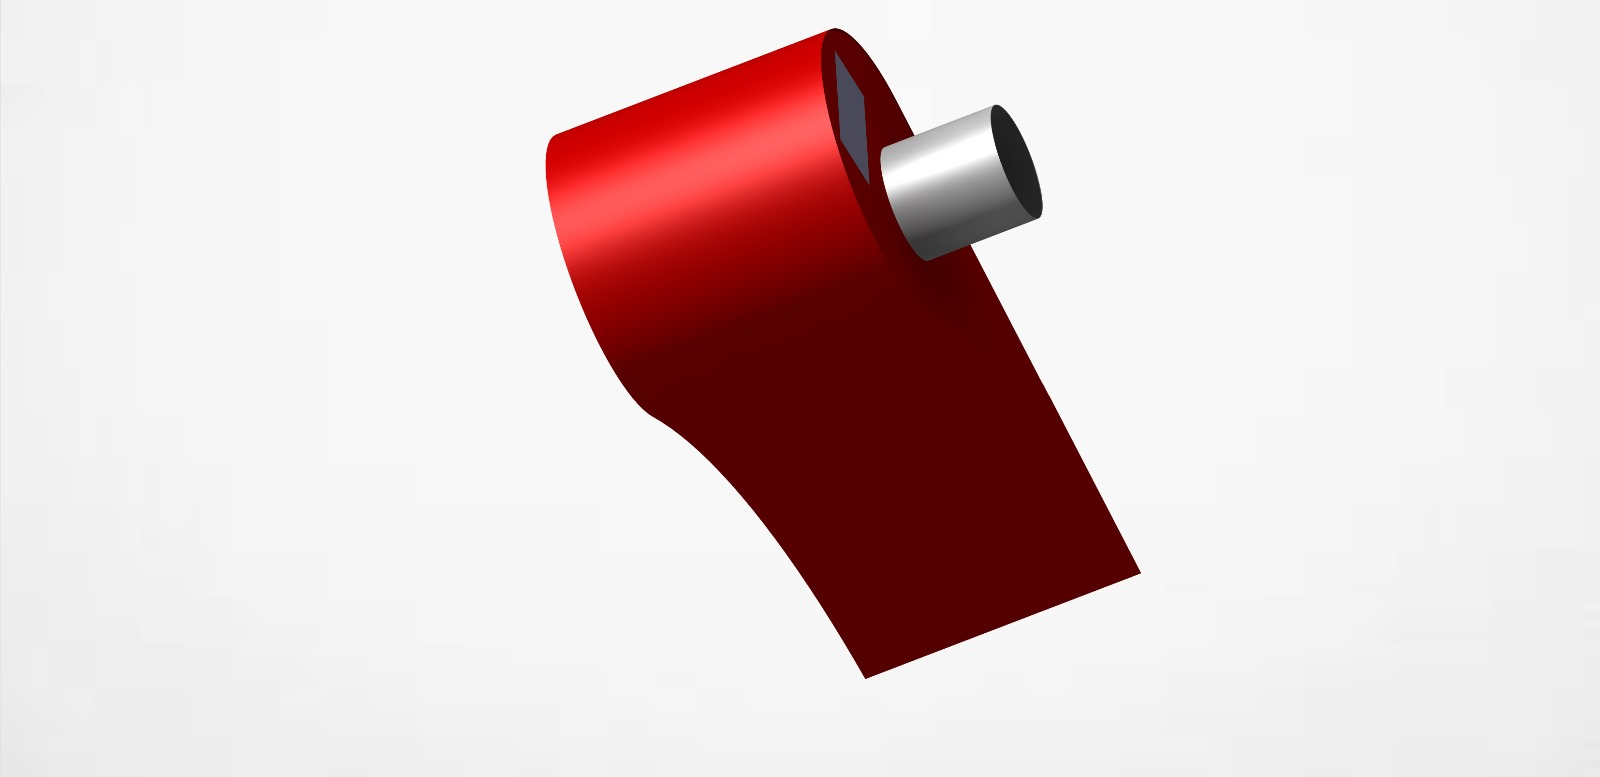
\includegraphics[width=2cm]{Figures/Montaje/14.jpg}}; \\
 };
\draw[marr] ([xshift=1mm]img-l.south west) coordinate (aux) 
 -- (img-m.north-|aux);
\draw[marr] (img-m) -- (img-n);
\end{tikzpicture}
\caption{Decimotercer Paso. \label{fig:dete}}
\end{figure}
%===============================================================================================================


\subsection{Decimocuarto paso: Revestimiento del Intradós}
El procedimiento del paso anterior se repite para el intradós, pero procediendo con un remachado ciego, al no contar con acceso por las dos partes.

Ver figura \ref{fig:decic}.
%===============================================================================================================
%                                                   14º PASO
%===============================================================================================================
\begin{figure}[!htb]
\centering
\begin{tikzpicture}[lablum/.style 2 args={label=below:#1 #2,name=img-#1},
marr/.style={line width=1mm,-latex}]
 \matrix[column sep=1cm,row sep=5mm] (mat)
 { \node[lablum=l]{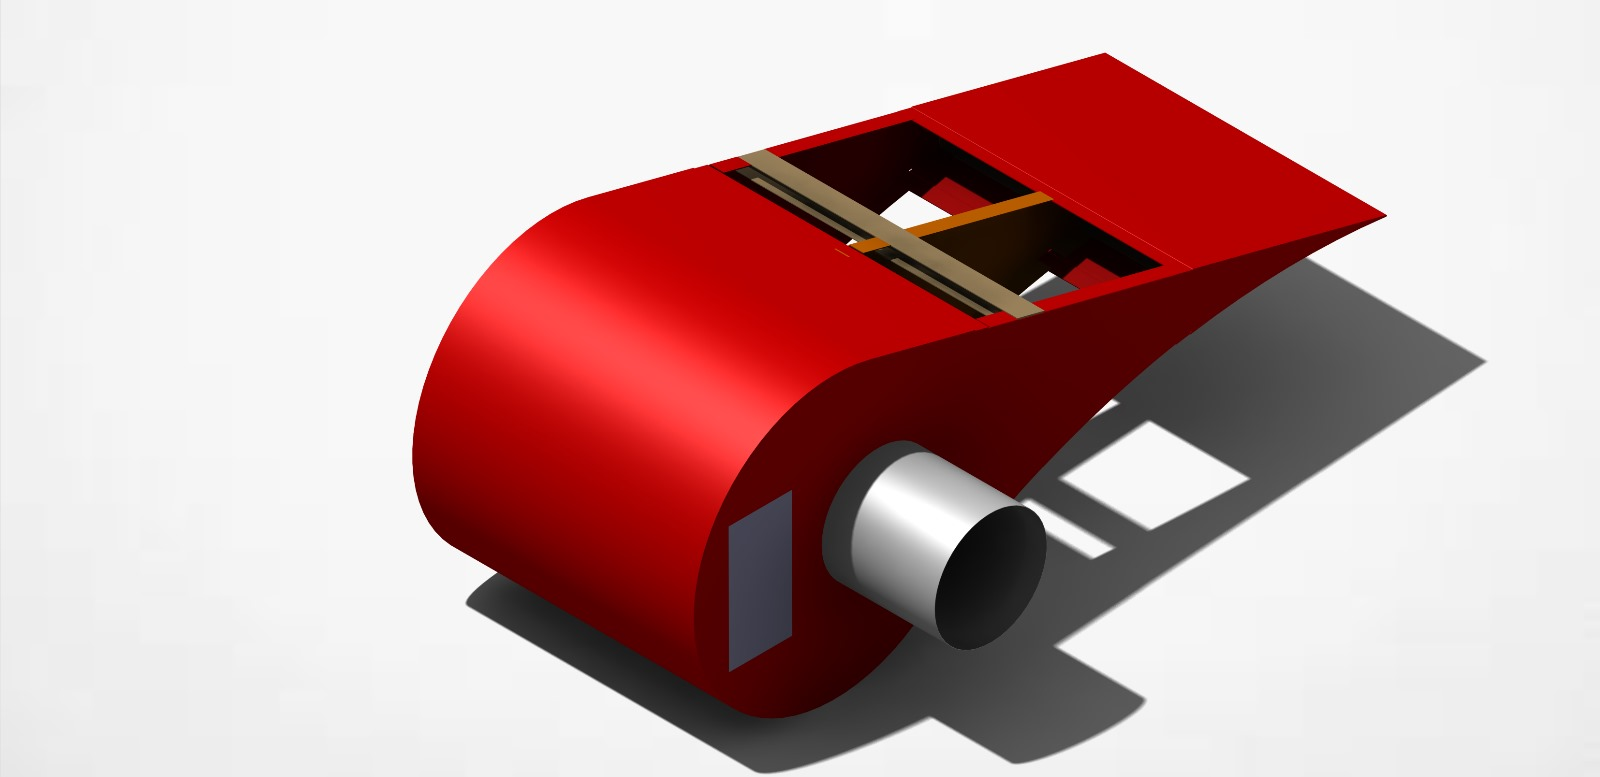
\includegraphics[width=2cm]{Figures/Montaje/12.jpg}}; &  \\
 \node[lablum=m]{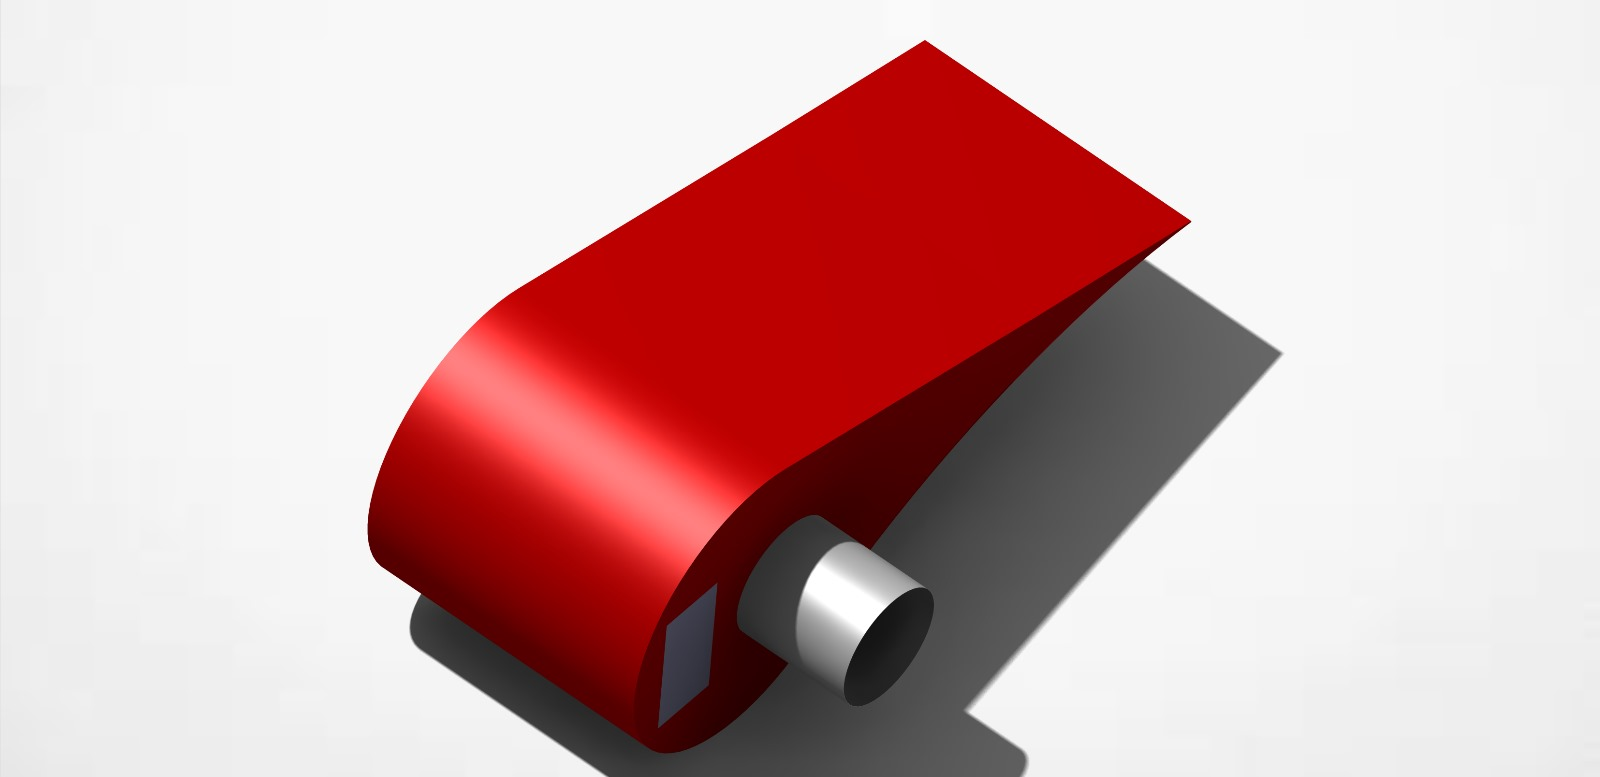
\includegraphics[width=2cm]{Figures/Montaje/13.jpg}}; & \node[lablum=n]{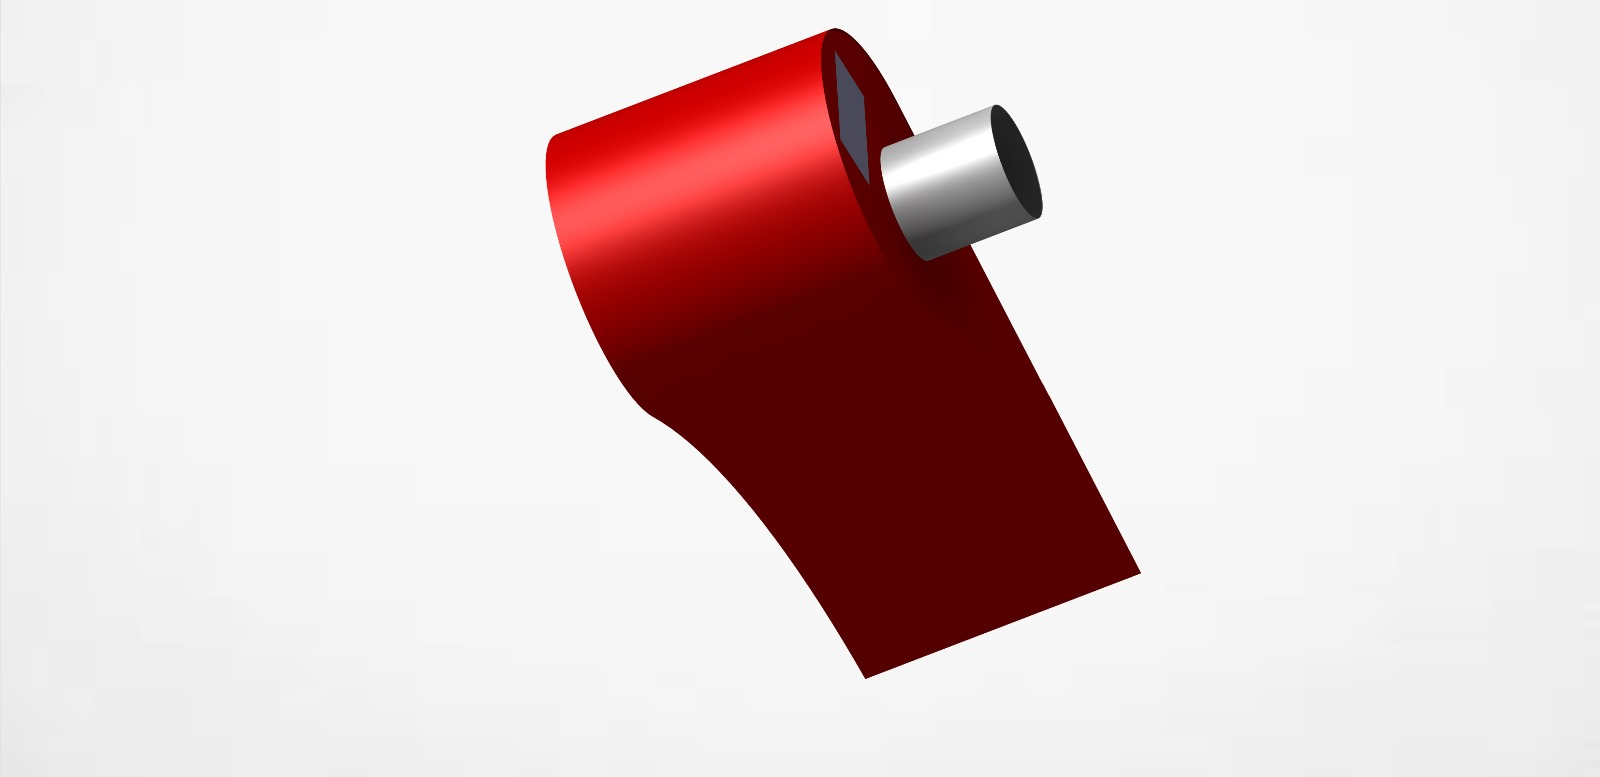
\includegraphics[width=8cm]{Figures/Montaje/14.jpg}}; \\
 };
\draw[marr] ([xshift=1mm]img-l.south west) coordinate (aux) 
 -- (img-m.north-|aux);
\draw[marr] (img-m) -- (img-n);
\end{tikzpicture}
\caption{Decimocuarto Paso. \label{fig:decic}}
\end{figure}
%===============================================================================================================

\pagebreak
\section{Proceso Global}
El proceso global se detalla en la figura \ref{fig:montaje}

%===============================================================================================================
%                                                   PROCESO GLOBAL
%===============================================================================================================
\begin{figure}[!htb]
\centering
\begin{tikzpicture}[lablum/.style 2 args={label=below:#1 #2,name=img-#1},
marr/.style={line width=1mm,-latex}]
 \matrix[column sep=1cm,row sep=5mm] (mat)
 { \node[lablum={a}{}]{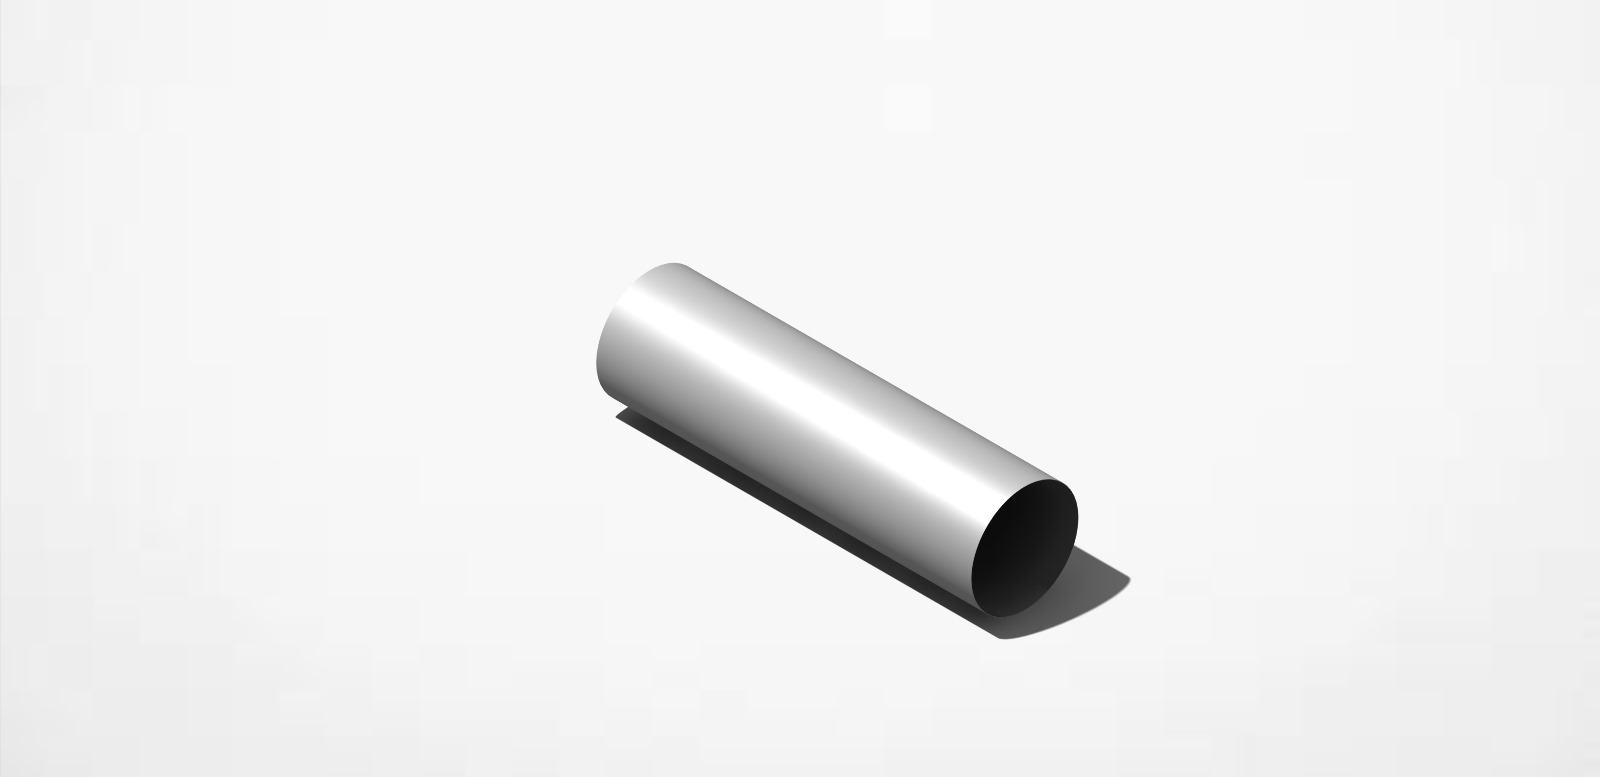
\includegraphics[width=4cm]{Figures/Montaje/1.jpg}};
 & \node[lablum={b}{}]{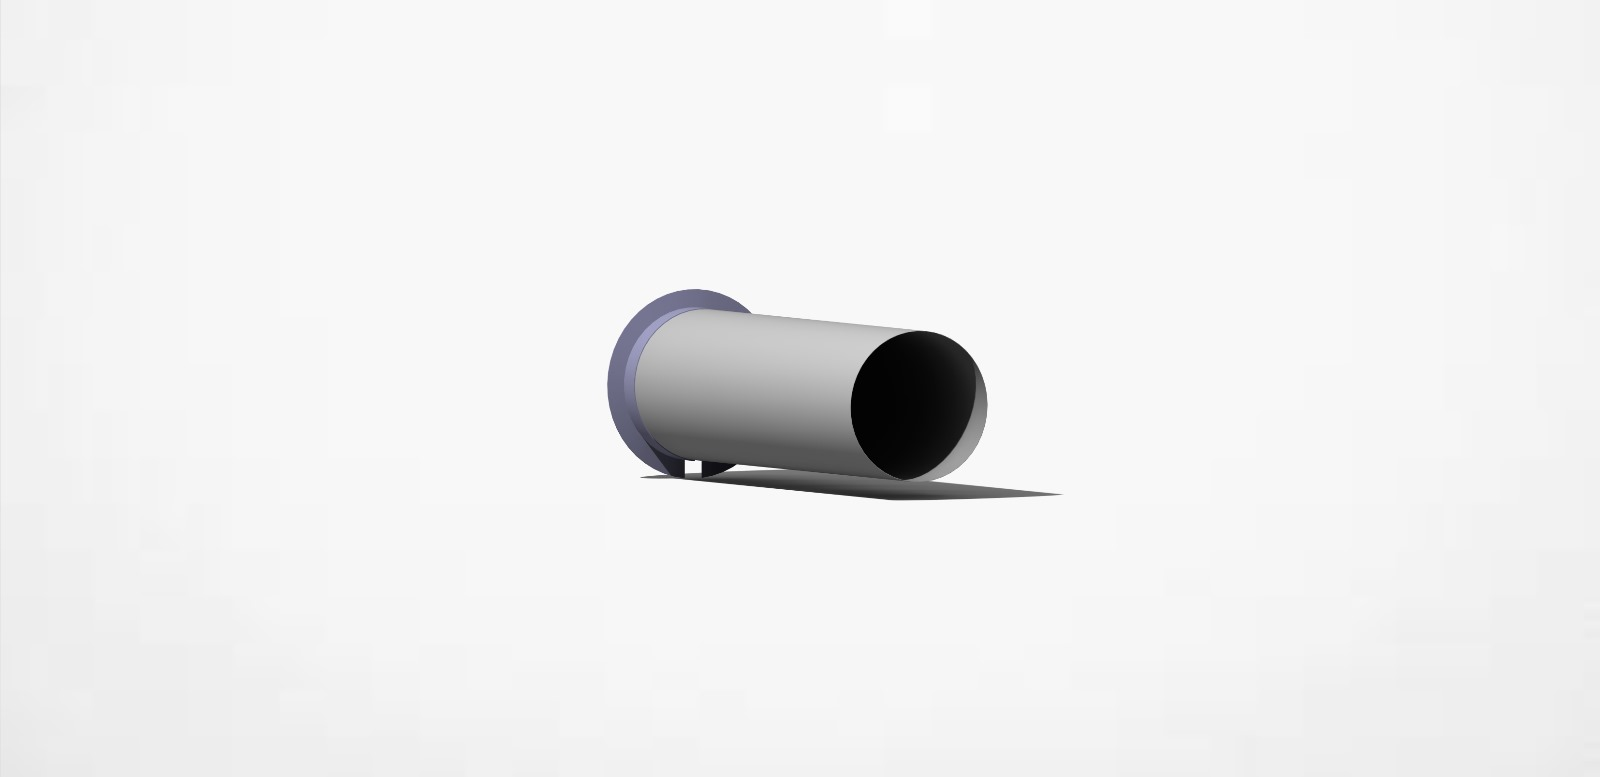
\includegraphics[width=4cm]{Figures/Montaje/2.jpg}};\\
 \node[lablum=d]{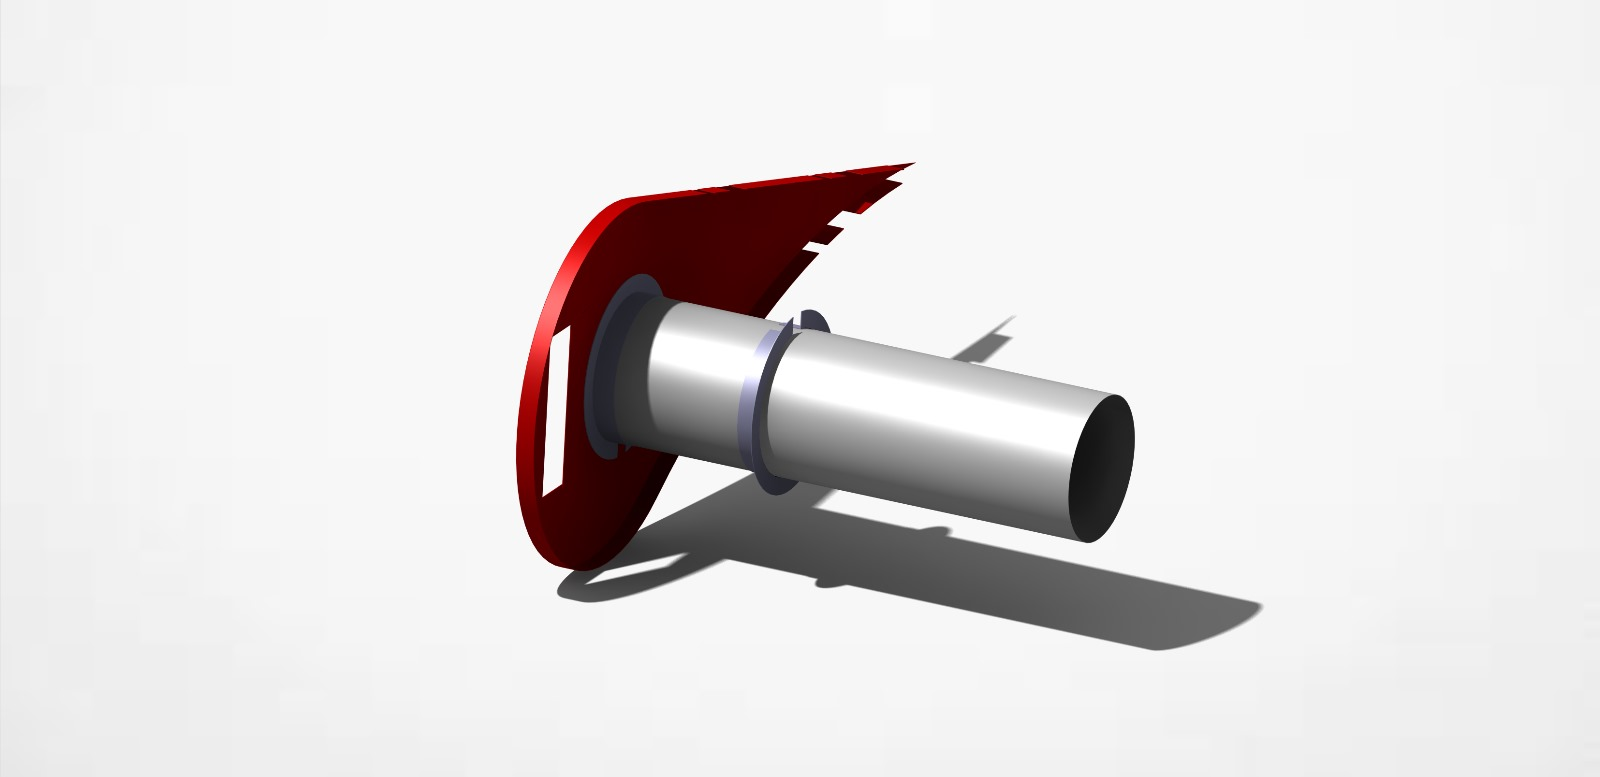
\includegraphics[width=4cm]{Figures/Montaje/4.jpg}};
 & \node[lablum=c]{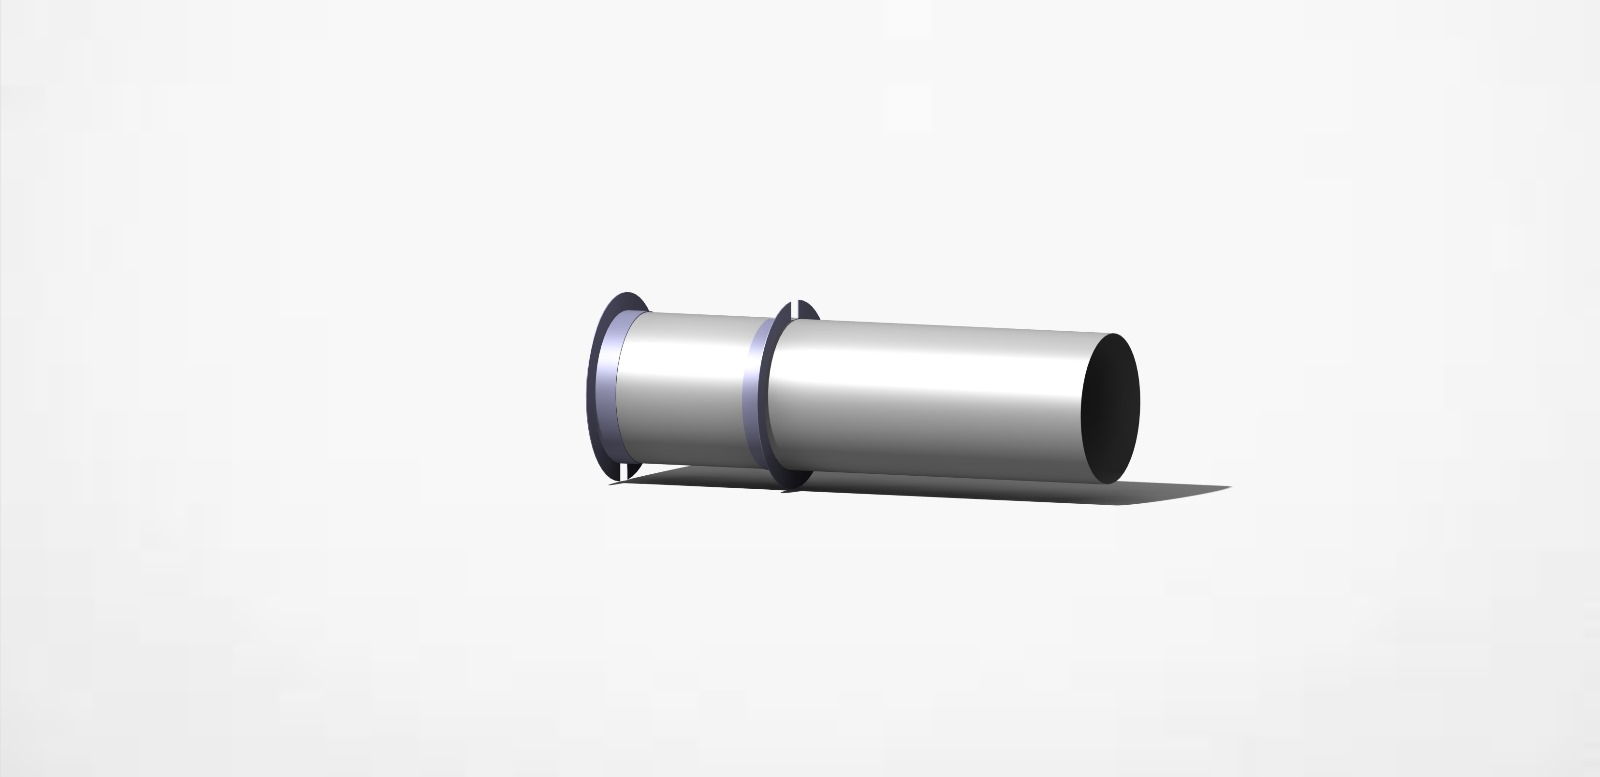
\includegraphics[width=4cm]{Figures/Montaje/3.jpg}};\\
 \node[lablum=e]{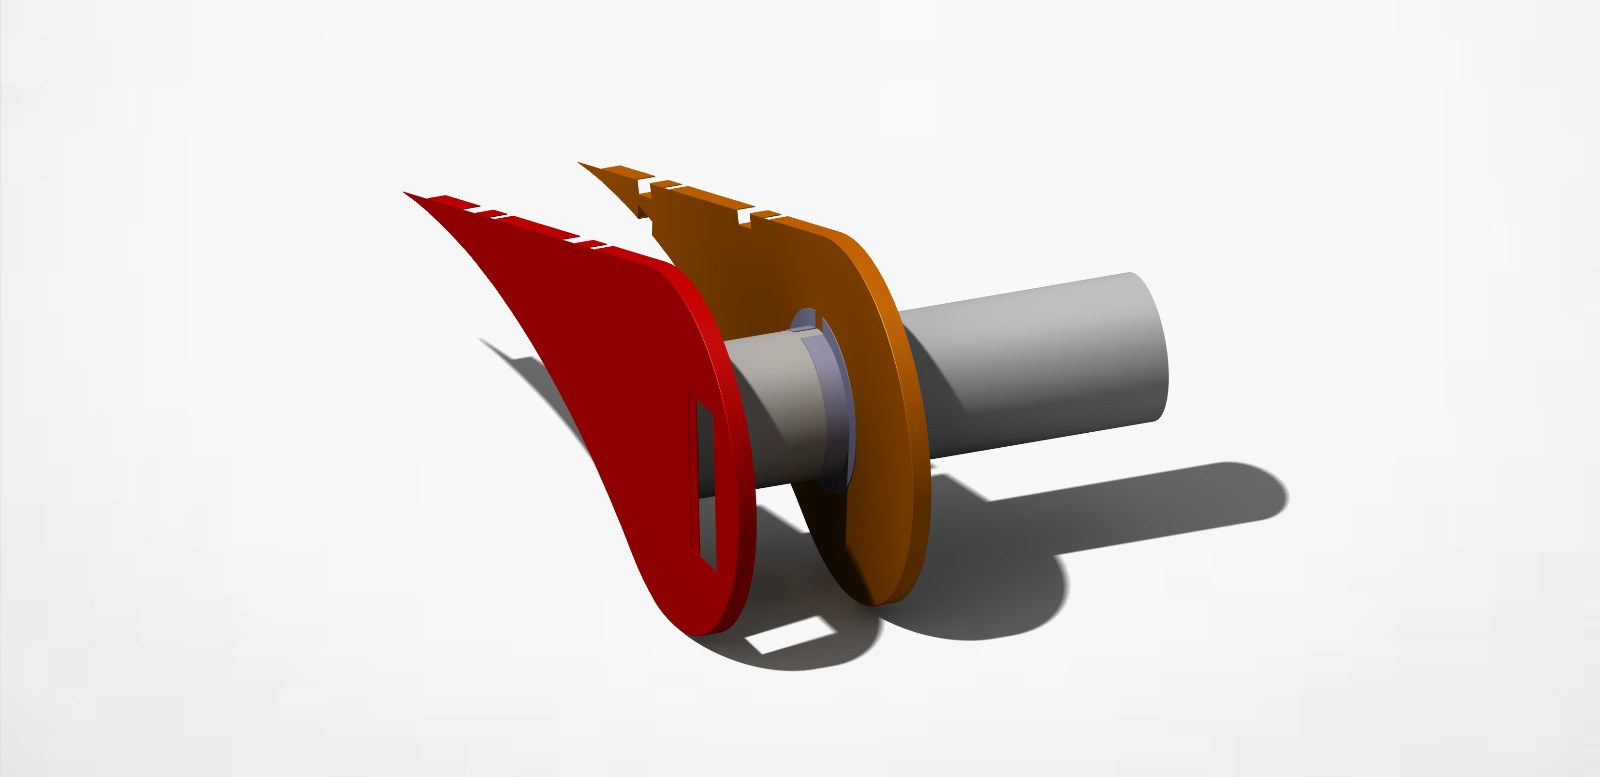
\includegraphics[width=4cm]{Figures/Montaje/5.jpg}};
 & \node[lablum=f]{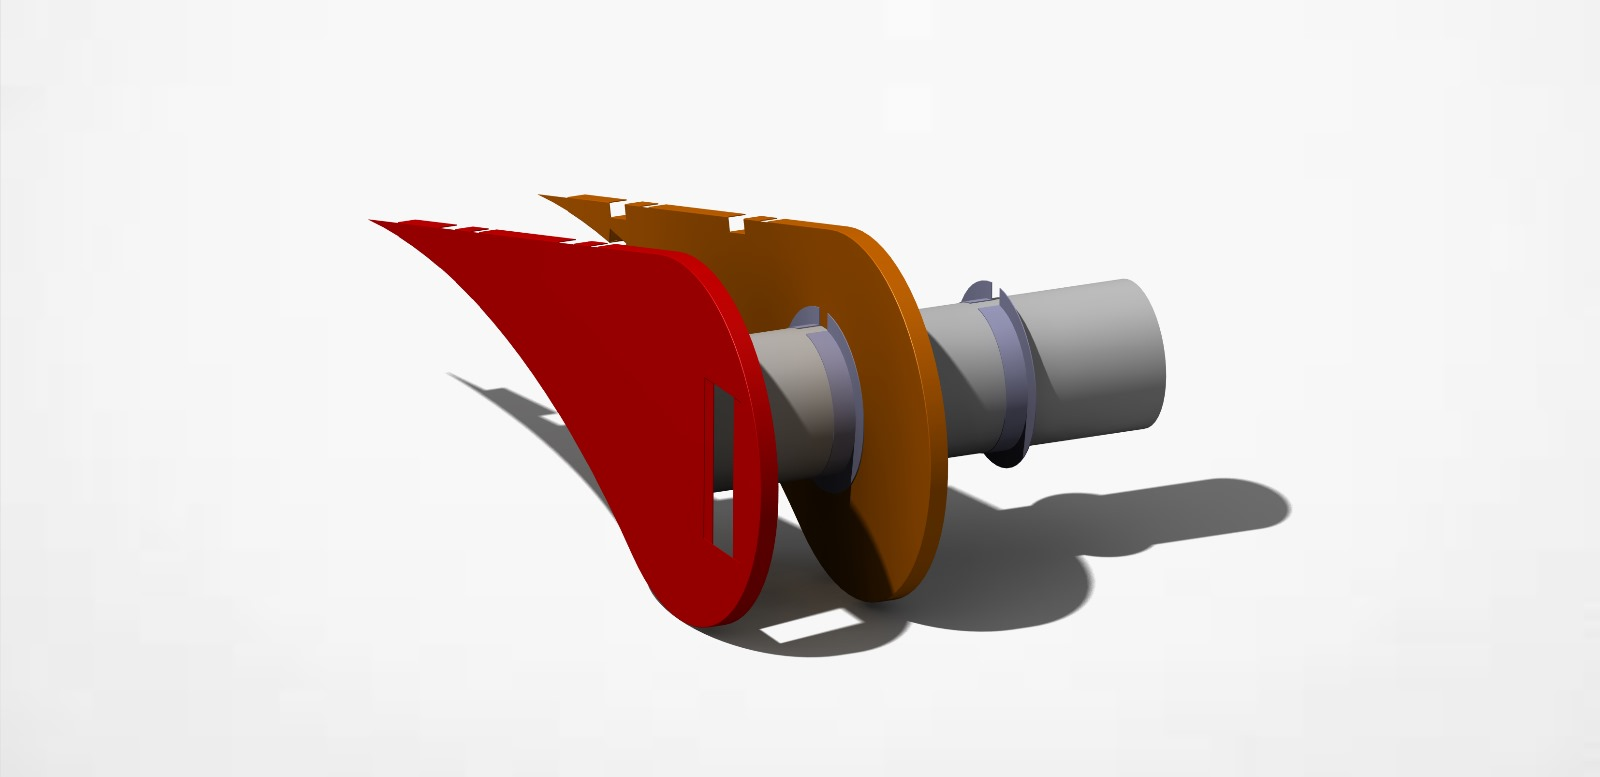
\includegraphics[width=4cm]{Figures/Montaje/6.jpg}};\\
 \node[lablum=h]{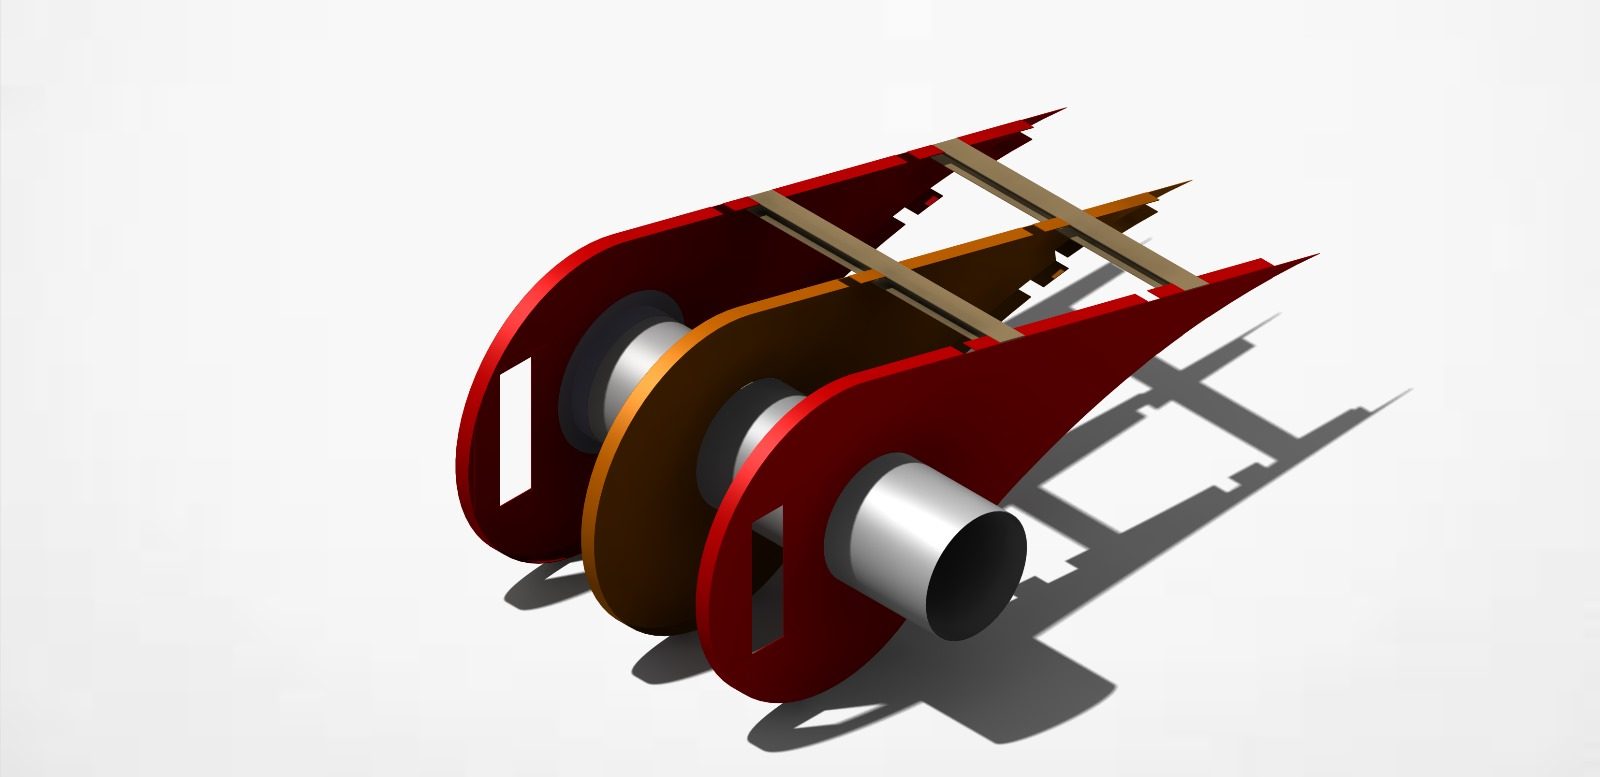
\includegraphics[width=4cm]{Figures/Montaje/8.jpg}}; & \node[lablum=g]{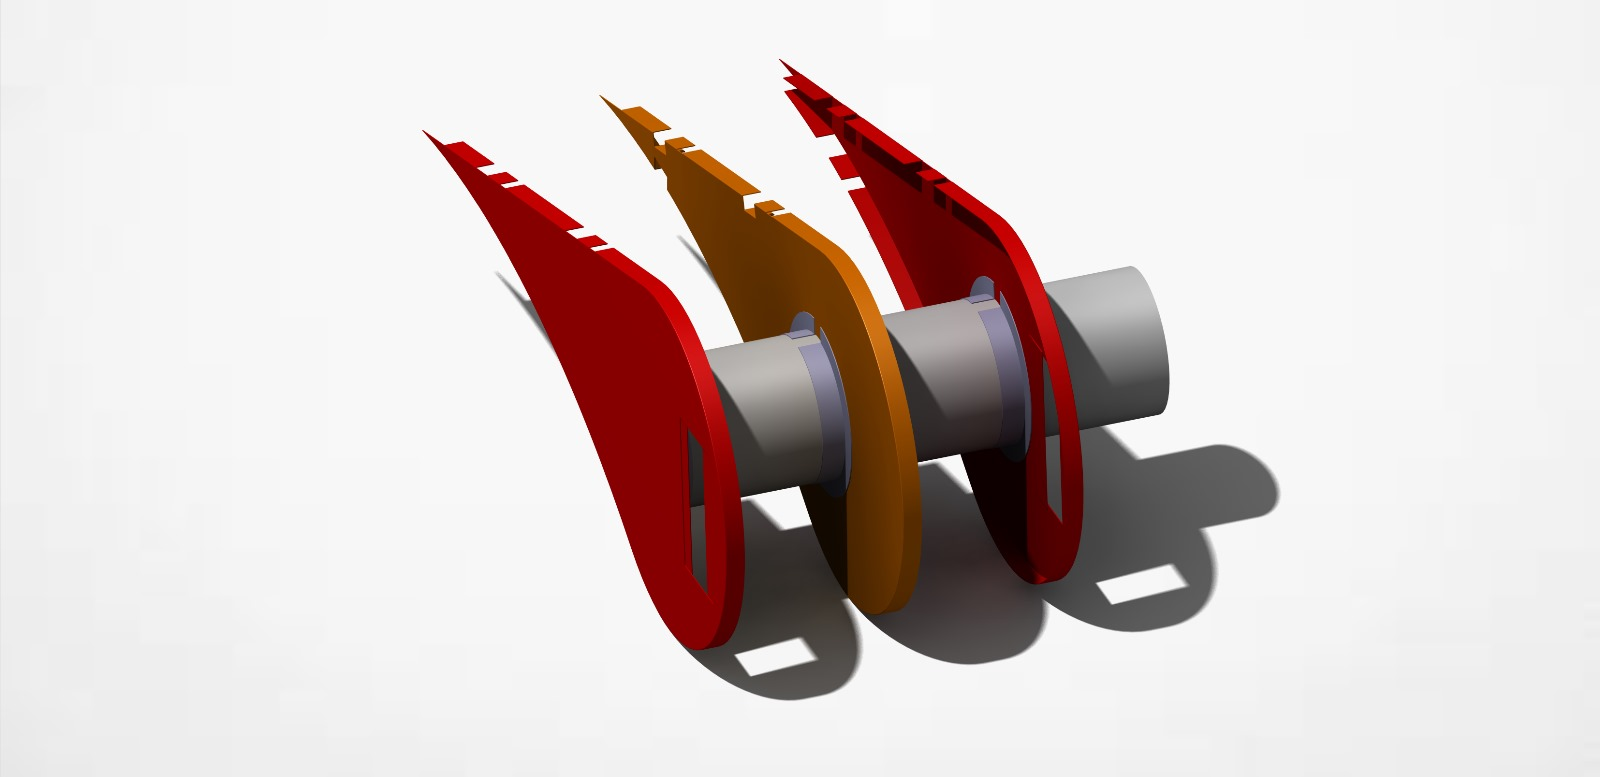
\includegraphics[width=4cm]{Figures/Montaje/7.jpg}};\\ 
\node[lablum=i]{\includegraphics[width=4cm]{Figures/Montaje/9.jpg}}; & \node[lablum=j]{\includegraphics[width=4cm]{Figures/Montaje/10.jpg}}; \\
\node[lablum=l]{\includegraphics[width=4cm]{Figures/Montaje/12.jpg}}; & \node[lablum=k]{\includegraphics[width=4cm]{Figures/Montaje/11.jpg}}; \\
\node[lablum=m]{\includegraphics[width=4cm]{Figures/Montaje/13.jpg}}; & \node[lablum=n]{\includegraphics[width=4cm]{Figures/Montaje/14.jpg}}; \\
 };
 % -------------------------------------------------
 \draw[marr] (img-a) -- (img-b);
 \draw[marr] ([xshift=1mm]img-b.south east) coordinate (aux) 
 -- (img-c.north-|aux);
 \draw[marr] (img-c) -- (img-d);
 \draw[marr] ([xshift=-1mm]img-d.south west) coordinate (aux) 
 -- (img-e.north-|aux);
 \draw[marr] (img-e) -- (img-f);
 \draw[marr] ([xshift=-1mm]img-f.south east) coordinate (aux) 
 -- (img-g.north-|aux);
\draw[marr] (img-g) -- (img-h);
 \draw[marr] ([xshift=1mm]img-h.south west) coordinate (aux) 
 -- (img-i.north-|aux);
\draw[marr] (img-i) -- (img-j);
 \draw[marr] ([xshift=-1mm]img-j.south east) coordinate (aux) 
 -- (img-k.north-|aux);
 \draw[marr] (img-k) -- (img-l);
  \draw[marr] ([xshift=1mm]img-l.south west) coordinate (aux) 
 -- (img-m.north-|aux);
 \draw[marr] (img-m) -- (img-n);
\end{tikzpicture}
\caption{Proceso de Montaje.  \label{fig:montaje}}
\end{figure}
%===============================================================================================================